%!TEX root = ../dissertation.tex
\chapter{Aperture effects in Stellar Mass Estimates}

\label{ch:acm}
\newpage

\section{Introduction}
\label{ch2_intro}

In this chapter we investigate methods of constraining the star formation histories and stellar masses of galaxies where galaxy spectra are available. In particular, we look at the largest galaxy catalog of estimated stellar masses, star formation rates and gas metallicities, the MPA-JHU catalog \citep{brinchmann_physical_2004, kauffmann_stellar_2003, tremonti_origin_2004}, obtained from spectra from the Sloan Digital Sky Survey (SDSS) Legacy Survey. The MPA-JHU catalog has, over the last decade and a half, been one of the most influential and widely-used catalogs in the fields of galaxy formation and evolution; the original catalog paper of \citet{kauffmann_stellar_2003} has been cited over a thousand times. Here we test a fundamental assumption of the catalog, which is that spectroscopic measurements of the central region of the galaxy yield sufficient information to constrain star formation histories and stellar masses for the galaxy as a whole.\\

The importance of galaxy star formation histories has been discussed in Sections \ref{questions} and  \ref{sec: results}. Crucial to analyzing these histories are accurate inferences of star formation rates and stellar masses from observed data. In particular, the stellar mass function, which is used to calibrate the parameters in simulations that seek to reproduce the star formation histories of galaxy populations, relies on accurate observational calibrations of stellar mass. In this spirit, I examine one of the most widely used stellar mass estimation methods; this method from \citet{kauffmann_stellar_2003} involves two spectral indicators and uses an aperture correction to account for the limited spatial resolution coverage of SDSS spectra. I investigate the robustness of this method using spatially resolved spectra from the Mapping Nearby Galaxies at Apache Point Observatory survey (MaNGA; \citealt{bundy_overview_2014}).\\

\subsection{The SDSS spectra}
\label{sdss spectra}

As introduced in Section \ref{sec: surveys}, SDSS has been conducting a coordinated imaging and spectroscopic survey since 2000 and is currently in its fourth phase of operation. The first two phases of the survey, SDSS and its extension SDSS-II, ran from 2000--2008 and took spectroscopy over approximately 8,000 square degrees of mostly the northern galactic sky 
ran between 2000-2008. It served as the primary database for the MPA-JHU catalog (\citealt{brinchmann_physical_2004, kauffmann_stellar_2003, tremonti_origin_2004}), whose final results were published in SDSS's Data Release 8 (DR8), 
which contains observed spectra of a little over 900,000 galaxies \citep{aihara11a}.\\

The imaging and spectroscopic data were observed using a 2.5 m telescope at the Apache Point Observatory (APO) in Sunspot, New Mexico. The imaging data was obtained by using a wide-field mosaic CCD camera and the spectroscopic data, using twin multi-object fiber spectrographs  \citep{smee_multi-object_2013}, all of which are mounted at the Cassegrain focus of the telescope. The imaging survey, which is carried out in drift-scanning mode using a 5 $\times$ 6 array of 2048 $\times$ 2048 pixel detectors, obtains photometry in the \emph{u, g, r, i} and \emph{z} bands. This broadband photometric data, after reduction and calibration, serves as the pool of data from which spectroscopic target selection is then done. The spectroscopic fiber plug-plates are aluminum plates which have holes drilled into them at positions decided upon by the target selection and the optical fibers are plugged into into these holes. They have a circular field-of-view of radius 1.49 degrees and during SDSS-I and -II were outfitted with 640 fibers, allowing for simultaneous observation of 640 spectra (mostly galaxy spectra and some which are reserved for standard and blank sky observations for calibration) in a 3 degree diameter field of view over the course of a single exposure.\\

The fiber diameter of the optical fibers was chosen with a view to maximize the signal-to-noise (S/N) ratio for an extended source, keeping in mind the sky conditions at APO. The optimal choice that was decided upon corresponds to a fiber diameter of 180 $\mu$m or 3''. The rest-frame wavelength range of the spectra at the median redshift is from 3500 \AA\ to 8500 \AA\ with a spectral resolution:\\ $$R = \frac{\lambda}{\Delta\lambda} \approx 2000.$$ The spectra are calibrated using observations of F stars in each 3 degree field.\\

SDSS imaging data and spectra have played a significant role in many discoveries in astronomy and cosmology over the last decade and a half. In addition to fundamental measurements of cosmological parameters and the study of distant quasars and stars in our own galaxy, the Main Sample of galaxies in SDSS-I and -II (\citet{strauss02a}) has informed much of the new understanding of galaxy properties that we have today. This 
new understanding has included the quantification of the 
bimodal nature of galaxy properties {\bf cites}, the relationship
between galaxy properties and environment {\bf cites}, and
how galaxy properties relate to the masses and other properties
of their host dark matter halos {\bf cites}. Key to many 
of these  works has been the use of new ways to estimate
star formation histories, stellar masses, and chemistry of 
stars in galaxies, including those found in the MPA-JHU 
catalog.
I discuss the catalog and the methods used to estimate these quantities in the following sections.\\

\subsection{The MPA-JHU Catalog}

The MPA-JHU catalog is the result of a collaborative effort between a group of researchers at the Max Planck Institute for Astrophysics and the John Hopkins University and was first constructed for the first SDSS Data Release (DR1) of spectroscopic observations. The original dataset they used was 120,808 galaxies drawn from the SDSS DR1 for which the following properties were estimated: stellar masses and mass-to-light ratios, effective stellar attenuation by dust, indicators of recent major starbursts, current total and specific star-formation rates, gas-phase metallicities, AGN classifications based on the standard emission line ratio diagnostic diagrams and AGN luminosities. The methods of estimation of these properties can be found in \citet{kauffmann_stellar_2003} for the stellar masses, \citet{brinchmann_physical_2004} for the star formation rates and \citet{tremonti_origin_2004} for the gas phase metallicities.\\

The MPA-JHU catalog measurements are ubiquitous in galaxy evolution literature with many important results relying on the inferred SFR's, masses and metallicities from the catalog. A few examples of scientific results from which the significance of the catalog can be evinced would be: understanding the host galaxies of AGN's by Kewley \citep{kewley2006}, the star formation-density relation and its reversal in distant universe by \citet{elbaz2007}, constraining the mass-metallicity relationship for star-forming galaxies \citep{kewley2008}, the mass dependence of radio-loud AGN's \citep{best05a}, insights into quenching mechanisms \citep{peng_mass_2010} and large scale galactic conformity \citep{kauffmann2013}, mapping the stellar mass function \citep{2009MNRAS.398.2177L, 2015MNRAS.454.4027D}, and many others.\\

The MPA-JHU catalog uses SDSS spectra to constrain the stellar masses and star formation histories in the catalog by looking at two key spectral indicators of starbursts and age of a galaxy: the Balmer ${\rm H}\delta_{\rm A}$ absorption line index and the ${\rm D}_{\rm n}4000$ break index.   Because they are both measurements defined over a narrow range of wavelengths in the blue, that are similar to each other, and are independent of the absolute flux, they are designed to be insensitive to dust extinction within the galaxy. The indices are discussed in detail in Sections \ref{d4000} and \ref{hdelta}. Using the distribution of the observed galaxies in the ${\rm H}\delta_{\rm A}-{\rm D}_{\rm n}4000$ plane and by employing Stellar Population Synthesis (SPS) models by \citet{bruzual_stellar_2003-1} to model the evolution of galaxies in this plane, they are able to derive maximum likelihood estimates of the stellar mass of a galaxy \citep{kauffmann_stellar_2003}, the attenuation of optical light by dust and the fraction of stars in a galaxy formed in recent bursts.\\

The spectra are only of the center of the galaxy so do not on their own constrain the total stellar mass. What is actually inferred from each spectrum at a given point ${\rm H}\delta_{\rm A}-{\rm D}_{\rm n}4000$ phase space is the mass-to-light ratio in the $z$-band for models that are at that same point. Now, as we have just seen in Section \ref{sdss spectra}, due to the nature of fiber spectroscopy, the angular area of coverage of a galaxy observed is limited to 3$''$, which could correspond to different actual physical sizes depending on the redshift of the galaxy. Thus, \citet{kauffmann_stellar_2003} (and in a similar way for SFRs, \citealt{brinchmann_physical_2004}) prescribe a method of aperture correction that relies on the assumption that the mass-to-light ($M/L$) ratio of the central part of a galaxy is representative of the entire galaxy. Thus the fiber M/L ratios are obtained in the \emph{z}-band are multiplied by the luminosity of the galaxy in the \emph{z}-band, that can be obtained from SDSS broadband photometry accounting for 
the full flex of the galaxy and thus presumably the 
total stellar mass of the galaxy. The methodology and the motivations behind it are discussed in further detail in Section \ref{kauffmann method}.\\

It follows from the above that the MPA-JHU catalog stellar 
masses would be systematically affected whenever the 
central $M/L$ ratios were not representative of the 
entire galaxy. For example, the bulge and disk components
of luminous spiral galaxies have systematically different
star formation histories and thus mass-to-light ratios; 
since the bulge dominates the inner part of the galaxy,
it can potentially dominate the fiber spectrum and yield
a $M/L$ unrepresentative of the galaxy as a whole.
To quantify exactly how this systematic affects
MPA-JHU masses  spatially resolved spectra for galaxies
is necessary.
Integral Field Unit (IFU) based surveys provide us the 
necessary data to be able to do that. In the following
section, I review briefly  the field of integral field spectroscopy and describe in more detail the MaNGA survey
\citep{bundy_overview_2014}.

\subsection{Integral Field Spectroscopy and MaNGA}

Integral Field Spectroscopy in astronomy is motivated
by the need to study the variation of spectra across
extended objects, in order to determine its internal
structure and dynamics.
An Integral Field Unit (IFU) enables the observation 
of multiple regions of the extended object simultaneously 
to obtain these spatially resolved spectra. There are many 
ways of doing this, including and not limited to image 
slicers, lenslet arrays, and multi-fiber IFUs. As we 
have seen in Section \ref{sdss spectra}, while 
spectroscopic surveys have created huge breakthroughs 
in galaxy evolution and cosmology alike, their restricted 
spatial coverage has resulted in the need for more or 
less uncertain aperture corrections to measure properties
of the galaxy as a whole, and in the inability to 
make reliable inferences about galaxies' internal structure.

Some noteworthy IFU-based surveys include the 
Sydney-Australian-Astronomical-Observatory Multi-object Integral-Field Spectrograph (SAMI; \citealt{bryant_sami_2015}), the 
Multi Unit Spectroscopic Explorer (MUST; \citealt{bacon_muse_2015}), and the Calar Alto Legacy 
Integral Field Area Survey (CALIFA; \citealt{sanchez_califa_2012}). 
Over the last decade these and other surveys have
contributed greatly to our understanding of the internal 
lives of galaxies. 
For the purposes of this project, 
the survey that bests suits our purposes is 
MaNGA (Mapping Nearby Galaxies at Apache Point \citep{bundy_overview_2014}). MaNGA is the largest 
IFU-based survey undertaken so far in terms of 
numbers of galaxies, planning to obtain spatially 
resolved spectra of about 10,000 galaxies by 2020. 
This size and the homogeneous selection of 
galaxies is one important consideration 
(Section \ref{mangadrp}). Another important 
consideration is that it uses the BOSS spectrograph,
which is very similar to the original SDSS spectrograph,
and the data is calibrated and processed using very
similar methods to SDSS-I and -II data.
These properties make it a natural sample to use
to test systematics in the methods applied to 
the MPA-JHU catalog.

MaNGA uses 17 multiple fiber IFUs simultaneously
\citep{drory_manga_2015}.
In the same way that single fibers are plugged into 
plates (Section \ref{sdss spectra}), the multiple 
fiber bundles are plugged at the appropriate 
locations on plug-plates to be observed at the 
focal plane of the 2.5m telescope at Apache Point. 
The fibers are 2.0$''$ in size and the bundles 
themselves come in five sizes and contain 19, 
37, 61, 91 or 127 fibers. The bundle assigned to 
each galaxy is determined from the 
angular size of the target galaxy. 

The fibers are arranged in a hexagonal pattern, 
and several observations are taken slightly offset 
from each other (``dithered'') to produce a denser 
hexagonal sampling. During data processing, the 
observations are interpolated onto a rectangular 
grid at each wavelength. 
Each grid point is called a spaxel, which can be 
thought of as a spectrum for every two-dimensional 
pixel. The resulting MaNGA galaxy outputs are 
thus three dimensional ``datacubes" with two 
spatial dimensions and one spectral dimension. 

Each bundle also contains sky fibers to allow for 
very precise sky subtraction by looking at a region of 
the sky that is within a few arcminutes of the target. 
At a given time, MaNGA is able to target 17 galaxies 
(and 12 standard stars) in the 3 degree FOV with much 
wider and continuous wavelength coverage than other
large IFU-based surveys.\\

\section{The $H\delta_{\rm A}-D_{\rm n}4000$ plane}
\label{indices}

In this section, I review the two spectral diagnostic tools used by the MPA-JHU catalog to constrain stellar masses and star formation histories in galaxies, the Balmer $\delta$ absorption line index and the ${\rm D}_{\rm n}4000$ break index in the optical spectrum of a galaxy. Following that I describe the method used by \citet{kauffmann_stellar_2003} to obtain the mass-to-light ratios of galaxies using these indices and finally the aperture correction method used to tranform the fiber masses obtained to the total stellar mass of the galaxy.\\

\subsection{The $D_{\rm n}4000$ break in Galaxy Spectra}
\label{d4000}

Spectral discontinuities in stars can be 
produced by the accumulation of a large number 
of spectral lines in a narrow region. 
In certain cases this can lead to a relatively 
sharp discontinuity, or ``break,'' in  the 
spectrum of the star.  
A prominent break in galaxy spectra occurs in the
optical at 4000 
\AA \citep{bruzual1981, bruzual_a._spectral_1983}, 
which exists in the spectra of K stars and thus 
appears in stellar populations older than a few
billion years, which are dominated
by K giants. Because it is associated with this 
late stage in the evolution of stellar populations,
the strength of this break is an indicator of the 
mean stellar age over the past few billion years.

The specific metallic absorption lines causing the break 
include a variety of elements in varying states of 
ionization, including including the CaII doublet, H 
and K (3969 \AA and 3934 \AA)
\citep{hamilton1985}. The stellar break strength
correlates positively with stellar metallicity, which
means that for galaxies the break exhibits some of the 
same age-metallicity degeneracy that afflicts most spectroscopic indicators.\\ 

%The so-called 4000 \AA\ break is produced by the absorption of metallic lines of a variety of elements in various states of ionization,  The opacity suddenly increases for photons bluer than this wavelength, which produces an intensity drop. It is enhanced in old stellar populations, which tend to be metal rich, but it is also present in younger galaxies.

%The most obvious discontinuity in the spectrum of a galaxy is often the $D_{n}4000$ break \citep{1999ApJ...527...54B}, which is a consequence of the absorption into electronic excited states by neutral and partially ionized metals whose lines happen to overlap in the region just blueward of 4000 \AA.  Older stellar populations have spectra dominated by relatively cool giant stars, and under these conditions the partially ionized metal lines are strong. Younger stellar populations have spectra dominated by hot stars, for which these lines are weaker. 

This break was defined in by \citet{bruzual_a._spectral_1983-2} as the 
ratio of the average flux density $F_{\rm \nu}$ in two bands that span 
\textasciitilde200 \AA\ on either side of 4000 \AA. 
\citet{1999ApJ...527...54B} defined a narrow bandwidth for
the break (known as $D_n$4000), using 100 \AA\ wide bands for
the blue (3850--3950 \AA) and red (4000--4100 \AA).
\citet{kauffmann_stellar_2003} 
(Figure \ref{fig:early_late_type}) uses $D_n$4000, because
it is less sensitive to dust reddening effects. In this 
section, I will use the same narrow band definition.\\

%\begin{figure}
%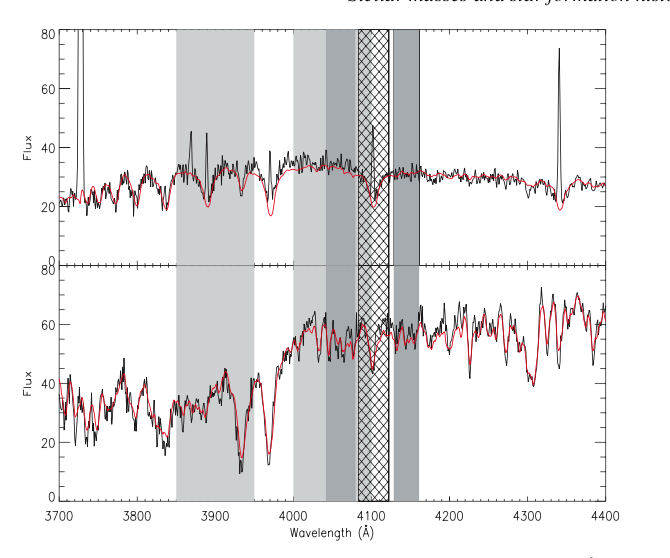
\includegraphics[width=\textwidth]{figures/spectra_placeholder.png}
%\caption[PLACEHOLDER FIG; TBD: A figure showing D4000 and Hdelta breaks in spectra for early/late-type galaxies as well as the bimodality in D4000
%]{ PLACEHOLDER FIG; TBD: A figure showing D4000 and Hdelta breaks in spectra for early/late-type galaxies as well as the bimodality in D4000
%\label{fig:early_late_type}}
%\end{figure}


\begin{figure}
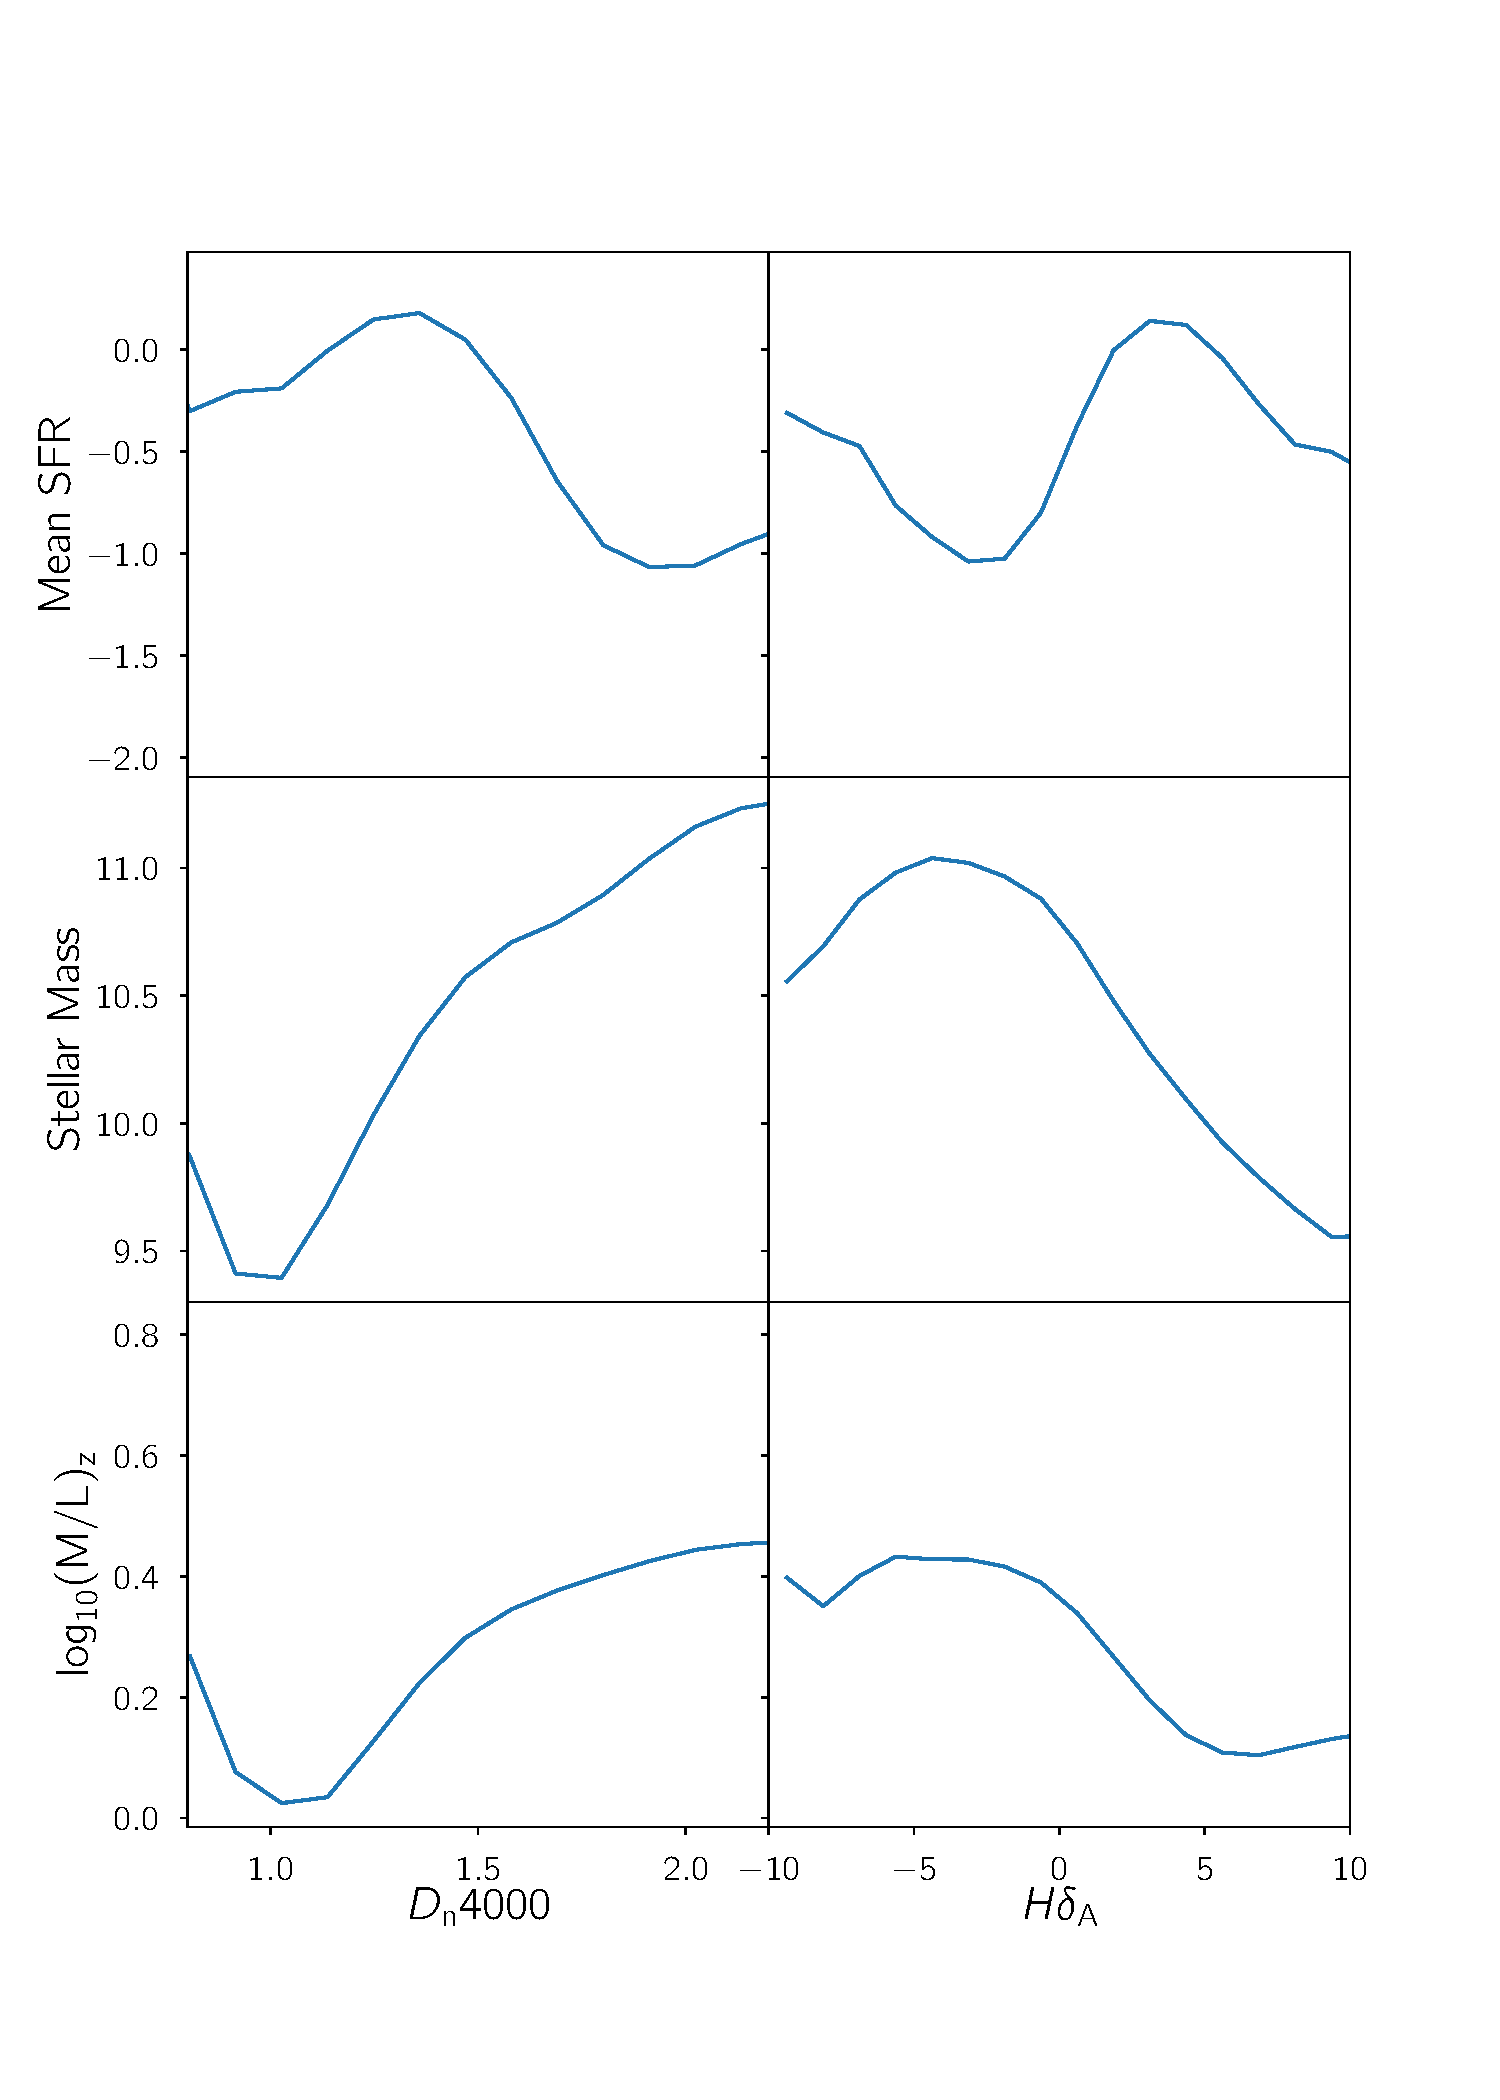
\includegraphics[width=\textwidth]{figures/mass_age_sfr_dist.pdf}
\caption[SFR's, stellar masses, ages and Mass-to-light ratios as a function of H$\delta_{\rm A}$ and ${\rm D}_{\rm n}4000$ for the DR8 SDSS galaxies
obtained from the MPA-JHU catalog]
{Stellar masses, ages and Mass-to-light ratios as a function of H$\delta_{\rm A}$ and ${\rm D}_{\rm n}4000$ for the DR8 SDSS galaxies obtained from the MPA-JHU catalog
\label{fig:sfr_mass}}
\end{figure}


\subsection{The Balmer H$\delta$ Absorption Line}
\label{hdelta}

As we have seen in Section \ref{sed}, the spectral features of 
galaxies contain a wealth of information about their star 
formation properties. In stellar populations, the Balmer 
absorption lines (H$\alpha$, H$\beta$, $H\gamma$, $H\delta$, \ldots)
are indicative of the presence of A stars. The surface 
temperatures of these stars are cool enough that their photospheres
are not fully ionized, but hot enough that the $n=2$ state of
hydrogen is populated and thus the $2\rightarrow n$ transitions 
can cause absorption lines. The lifetimes of A stars are 0.5--1 
billion years, and therefore the strength of the Balmer
lines in galaxies is indicative of the relative fraction of star
formation that has occurred in the past few hundred million to
a billion years. For example, very strong H$\delta$ absorption 
in the absence of signatures of star formation indicates a 
a starburst having happened and ended 0.5--1.5 Gyrs ago 
\citep{1983ApJ...270....7D}. 

Like many spectroscopic indicators,
because the temperature of the stars is negatively correlated 
with metallicity, Balmer line indicators also suffer from an
age-metallicity degeneracy. However, this degeneracy can be 
broken with additional measurements of other features of the 
spectrum which have age-metallicity degeneracies that differ
in detail. Thus with the appropriate SPS models, both the 
mean age and metallicity can be simultaneously obtained. 
The traditional tool for this purpose is the set of Lick indices, 
obtained by using stellar spectra from the Lick Observatory 
\citep{1997ApJS..111..377W, worthey_comprehensive_1994}. The 
Lick indices are a system of 25 line indices, whose 
relationship to underlying stellar properties is thought
to be known. 

Here we will utilize these index measurements of the Balmer 
lines. Specifically we focus on H$\delta$. Although this absorption
line is weaker than the lower order lines, it is less contaminated.
The interstellar gas in galaxies is emitting Balmer recombination
lines. For H$\alpha$, $\beta$, and $\gamma$, the emission can 
be strong enough to swamp the absorption line in the 
continuum. 

Measuring these absorption feature indices involves measuring 
the flux in a central bandpass relative to two pseudo-continuum 
bandpasses on either side. The continuum from 
which the equivalent width is measured is defined by linear
interpolation between the midpoints  of the two flanking pseudo-continuum 
bandpasses. The bandpass definitions we use here, as defined 
by \citet{worthey_comprehensive_1994} are: an index bandpass from 
4083.50--4122.25 \AA\ with the blue and red bandpasses on either side 
being 4041.60--4079.75 \AA\ and 4128.50--4161 \AA\ respectively.

\subsection{Constraining SFH's using H$\delta_{\rm A}$ and $D_{\rm n}4000$}
\label{kauffmann method}

The MPA-JHU measurements of stellar masses and ages rely on the 
results concerning the evolution of the H$\delta_{\rm A}$ and 
$D_{\rm n}4000$ indices for stellar populations. The evolutionary 
tracks of these indices with age are mapped by the spectral library, 
STELIB, incorporated into the SPS models \citep{bruzual_stellar_2003} 
that are used to fit the SDSS spectral data. 
A significant prediction of these models here is that 
$D_{\rm n}4000$ is sensitive to the mean star formation rate over
time scales of billions of years, whereas the H$\delta_{\rm A}$ feature 
is sensitive to the mean star formation rate over hundreds of millions
of years. These features therefore provide constraints on the star
formation histories of the galaxies.

These observables are also related to metallicity, which means that
how they relate to star formation history is affected by the
age-metallicity degeneracy. However, the stellar mass-to-light ratio is 
also affected by this degeneracy in a similar fashion; therefore
a given value of these observables tends to correspond to the 
same $M/L$ even for different metallicity populations.

\citet{kauffmann2013} exploit these properties to constrain the 
stellar mass-to-light ratios of galaxies by using a Bayesian 
inference technique. The prior distribution is a library of models 
that are generated by Monte Carlo realizations that are 
representative of both bursty and continuous star formation 
histories. The library consists of 32000 different star formation 
histories, and provides predictions for each of the H$\delta_{\rm A}$ 
and $D_{\rm n}4000$ indices, the stellar mass-to-light ratios in the 
$z$-band, the $g-r$ and $r-i$ colors, and the fraction of stellar 
mass formed in bursts over the past 2 Gyr.\\

This library of models thus enables the construction of a 
``model grid" in the H$\delta_{\rm A}$-$D_{\rm n}4000$ plane,
where each point on the grid corresponds to a distribution of
physical properties of the models.
For each galaxy in SDSS DR8, the spectral indices are measured, 
and then the physical properties and their uncertainties inferred
from the distribution corresponding to those spectral index values.
% as emission line fluxes are calculated using a special purpose 
% code \citep{tremonti_origin_2004} that recovers the best fit 
% model spectrum for each galaxy based on the 
% \citet{bruzual_stellar_2003} SPS models. Thus for each galaxy 
%value of H$\delta_{\rm A}$ 
%and $D_{\rm n}4000$, along with an error estimate and can 
%now possibly be associated with a model from the library of 
%star formation histories. As the prior on the distribution of 
% the SFH's is akin to the parameter space being Monte Carlo 
% sampled, the likelihood of the distribution of the data 
% given the parameters can be assumed to be Gaussian. 
The resulting median value of the posterior probability distributions 
of the parameters for each galaxy is then used 
as the ``best" estimate in the catalog. The resulting 
mass-to-light ratios for the SDSS DR8 galaxies in the 
H$\delta_{\rm A}$-$D_{\rm n}4000$ plane thus obtained are 
plotted in Figure \ref{fig:kauff_grid}.\\ 

\begin{figure}
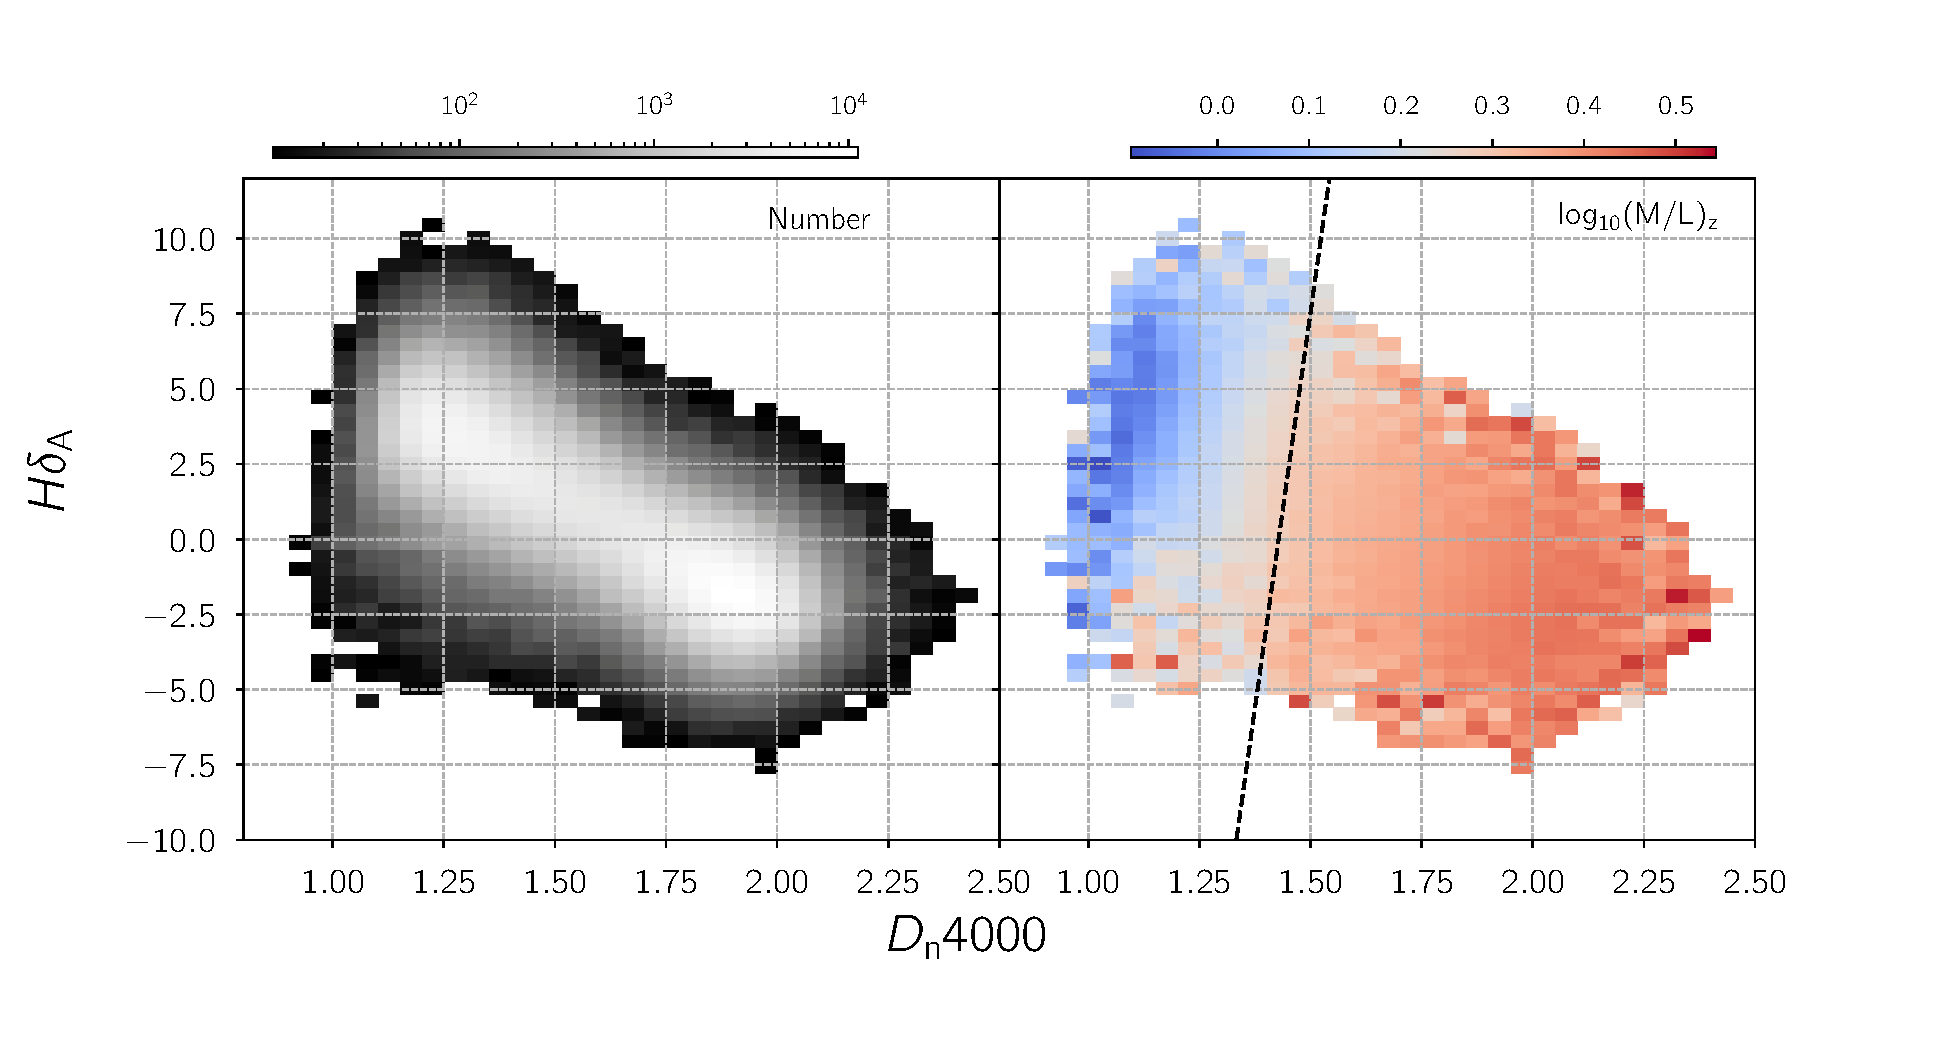
\includegraphics[width=\textwidth]{figures/hd_d4000_mlratio_coarser_binning.pdf}
\caption[The \citet{kauffmann_stellar_2003} grid to infer M/L ratios from the H$\delta_{A}-D_{n}4000$ plane; The grid was recreated using the MPA-JHU catalog for the SDSS DR8 galaxies. The line drawn here was chosen to distinguish between the younger and older populations; All the galaxies ``above" the line describe a ``younger" population and all the galaxies ``below", represent an older population.]
{The \citet{kauffmann_stellar_2003} grid to infer M/L ratios from the H$\delta_{A}-D_{n}4000$ plane; The grid was recreated using the MPA-JHU catalog for the SDSS DR8 galaxies. The line drawn here was chosen to distinguish between the younger and older populations; All the galaxies ``above" the line describe a ``younger" population and all the galaxies ``below", represent an older population.
\label{fig:kauff_grid}}
\end{figure}

\subsection{The Stellar Mass Aperture Bias in MPA-JHU}
\label{apercorr}

As we have reviewed in Section \ref{sdss spectra}, the SDSS spectra 
collect starlight within the 3$''$ fiber diameter, with fibers that 
have been placed as close to the centre of a galaxy as possible.
Thus mass-to-light ratios discussed above only strictly apply to the
center of the galaxies.
To obtain total stellar masses, the MPA-JHU catalog 
applies the mass-to-light ratio to the $z$-band photometry, using
a spectroscopically-determined correction for dust extinction.
These procedures assumes that the fiber mass-to-light ratios and 
dust attenuation factor is applicable to the whole galaxy. This
assumption could in principle be a source of systematic error,
i.e. an  aperture bias, as discussed in \citet{kauffmann_stellar_2003} 
(and \citet{brinchmann_physical_2004} for the star formation rates).\\
For example,  spiral galaxies with star forming outer discs could have 
the index measurements in the central bulge not reflective of the 
galaxy's star formation properties as a whole at all. 

\citet{kauffmann_stellar_2003} attempt to address this 
bias by comparing galaxies with similar z-band luminosities 
at different redshifts, using the fact that the physical
size of the aperture will depend on distance,
to see how significant the shift in ${\rm D}_{\rm n}4000$,
$(M/L)_{z}$ and $A_{z}$ are. They find that ${\rm D}_{n}4000$ 
and $A_{z}$ show a marked trend with redshift for galaxies 
whose absolute magnitude in z-band is between 
$-22.5 < M_{z} < -22.0$  but not for the galaxies that are 
brighter or fainter than that. The trends for $(M/L)_{z}$ are 
similar but less pronounced. However, even at the outer limit 
of the redshifts probed, the median fraction of total light 
from a galaxy entering the fiber is only half the total, and 
so bias in the true global $(M/L)_{z}$ of the galaxies in the catalog 
is not measured by this technique. 

The stellar mass estimates in the MPA-JHU catalog are 
certainly affected by other systematic effects, most
prominently the choice of the stellar IMF (which can cause 
a factor of two issue), but also the stellar population 
model choice, the choice of the star formation history prior 
(i.e., the model library), and other effects. These sorts
of biases have been explored in detail by other researchers
(see \citealt{conroy_modeling_2013} and references therein).
However, before this work there was not yet a direct 
demonstration that the aperture bias in these estimates 
was tolerable.

% In the companion paper of \citet{kauffmann2013}, \citet{brinchmann_physical_2004}, which deals with estimating star formation rates and specific star formation rates for the MPA-JHU catalog, an aperture correction is proposed for the estimated SFR's. Their aperture correction entails constructing likelihood distributions for SFR/$L_{i}$  based on the $g-r$ and $r-i$ colors, where $L_{i}$, the \emph{i}-band luminosity, serves as a proxy for the mass of the galaxy. These are then used to infer the total galaxy SFR's from the fiber SFR's. It is explicitly stated by the authors of \citet{brinchmann_physical_2004} that one of the significant sources of systematic error in the SFR estimates would have to be the orientation of the aperture and that one would need to model spatially resolved spectra to be able to truly verify the validity of the aperture corrections.\\

IFU-based surveys that cover a large fraction of each
galaxy's area are ideal to test the aperture 
effects on both SFRs and stellar masses in the MPA-JHU 
catalog. Therefore, in this chapter I investigate the aperture 
effects on the stellar mass estimates by using spatially 
resolved spectral data from MaNGA.\\


\section{Data and Methods}

\subsection{MaNGA Target Selection}
\label{mangadrp}

We use the MaNGA data set for two reasons. First,
its spectra have very similar properties to that of 
the original SDSS sample, with similar wavelength 
ranges and resolution. Second, its IFU data covers 
a large fraction of each galaxy, typically yielding 
a more global picture of each galaxy than obtainable
from other surveys. 

The MaNGA target selection is based on NSA photometry of 
SDSS Main Sample galaxies. The selection is designed to 
sample in a recoverable way as a function of stellar mass
and redshift, that in combination with the chosen fiber 
bundle sizes provide sufficient radial coverage as 
described  in the next paragraph.
The optimization process used to do this is described 
in \citet{2017AJ....154...86W}. MaNGA's goal is to 
observe approximately 10,000 galaxies by mid-2020,
the end of SDSS-IV.

MaNGA radial coverage goals are to cover the galaxy 
well beyond its effective radius, $R_{e}$ (the radius 
within which half of the galaxy's light is contained). 
There are three samples, the Primary, the Secondary, 
and the Color-enhanced samples. The Primary and Secondary 
samples, which make up 47\% and 37\% of the total sample, 
differ in the extent of spaxel coverage, with the 
former providing spectra for $>$80\% of galaxies to 
beyond $1.5R_{e}$ and the latter providing spectra
for $>$80\% of galaxies to beyond $2.5R_{e}$.  
The cuts in redshift for both are chosen to ensure 
that there is a flat number density distribution of 
galaxies in the absolute i-band magnitude. The 
color-enhanced sample, which makes up about 16\% 
of MaNGA, fills in for the undersampled regions in 
the \emph{N-i}-$M_{i}$ plane by extending the 
redshift limits in the primary sample so that 
galaxy types such as red galaxies with low luminosity, 
the green-valley galaxies and the high luminosity 
star-formers are better represented in MaNGA.\\

\subsection{Our Sample}

We use MaNGA Product Launch 8 (MPL-$8$), 
announced in November $2018$, containing products 
based on galaxy and stellar library observations from 
March $2014$ through July $2018$.
It contains $950$ plates with $6779$ galaxy data cubes.
Out of these cubes, $6468$ are galaxies with measured 
NSA redshifts. These are representative of all the 
IFU sizes (19, 37, 61, 91 or 127 fibers per IFU) and 
span a redshift range up to $z = 0.15$.\\

For each galaxy observation, depending on the IFU 
bundle size, the MaNGA Data Redshift Pipeline 
(\citealt{law_data_2016}) creates a data cube with
spectra on a rectilinear grid with a spacing of 
0.5$''$, with each grid point known as a ``spaxel.'' 
The dimensions of the grid are aligned with north
($Y$) and east ($X$) on the sky.

\subsection{Variable Aperture Measurements}
\label{sec:chap2methods}
For any given data cube, we want to convert it into
a set of aperture spectra to 
simulate the spectra that the SDSS-I and -II
surveys would have observed through single 3$''$ fibers
at a given set of redshifts.

For any aperture radius $R$, we determine which 
spaxels fall within an aperture radius of $R$ 
arcseconds based on its angular distance from the 
cube center (which corresponds to the center of 
each galaxy). Then we sum the spaxels within radius $R$ 
to obtain the equivalent spectrum. Alternatively we 
can sum all of the spaxels to obtain a ``full aperture''
measurement. Strictly speaking this aperture is of
course not always full; however, for the required
coverage of $1.5R_e$, typically 70\%--80\% of the 
light is included (with the lower number for de Vaucouleurs
galaxies and the upper number for exponential galaxies;
\citealt{graham05a}).

% As each spaxel spans a width of 0.5'' in along the ``X" and ``Y" 
%direction, at any point $(x,y)$ in the IFU image, the distance in 
%arc-seconds of the centre of a spaxel from the central spaxel 
%$(x_{c},y_{c})$ in the IFU would be:
% $$ d = (r(x,y) - r(x_{c},y_{c})) = \sqrt{(0.5*x)^2 + (0.5*y)^2} $$

% Thus, for every spaxel in the IFU, where $d<=R$, that 
% part of the galaxy would fall within the aperture and hence, 
%we would include that spaxel in the measurement of whichever 
%spectral index. Using this, for instance, we can simulate the 
%SDSS fiber measurement, i.e.,  what the $1.5$" aperture 
%radius used in SDSS would see versus the total galaxy 
%or what we call a ``full aperture" measurement.

%\begin{figure}
%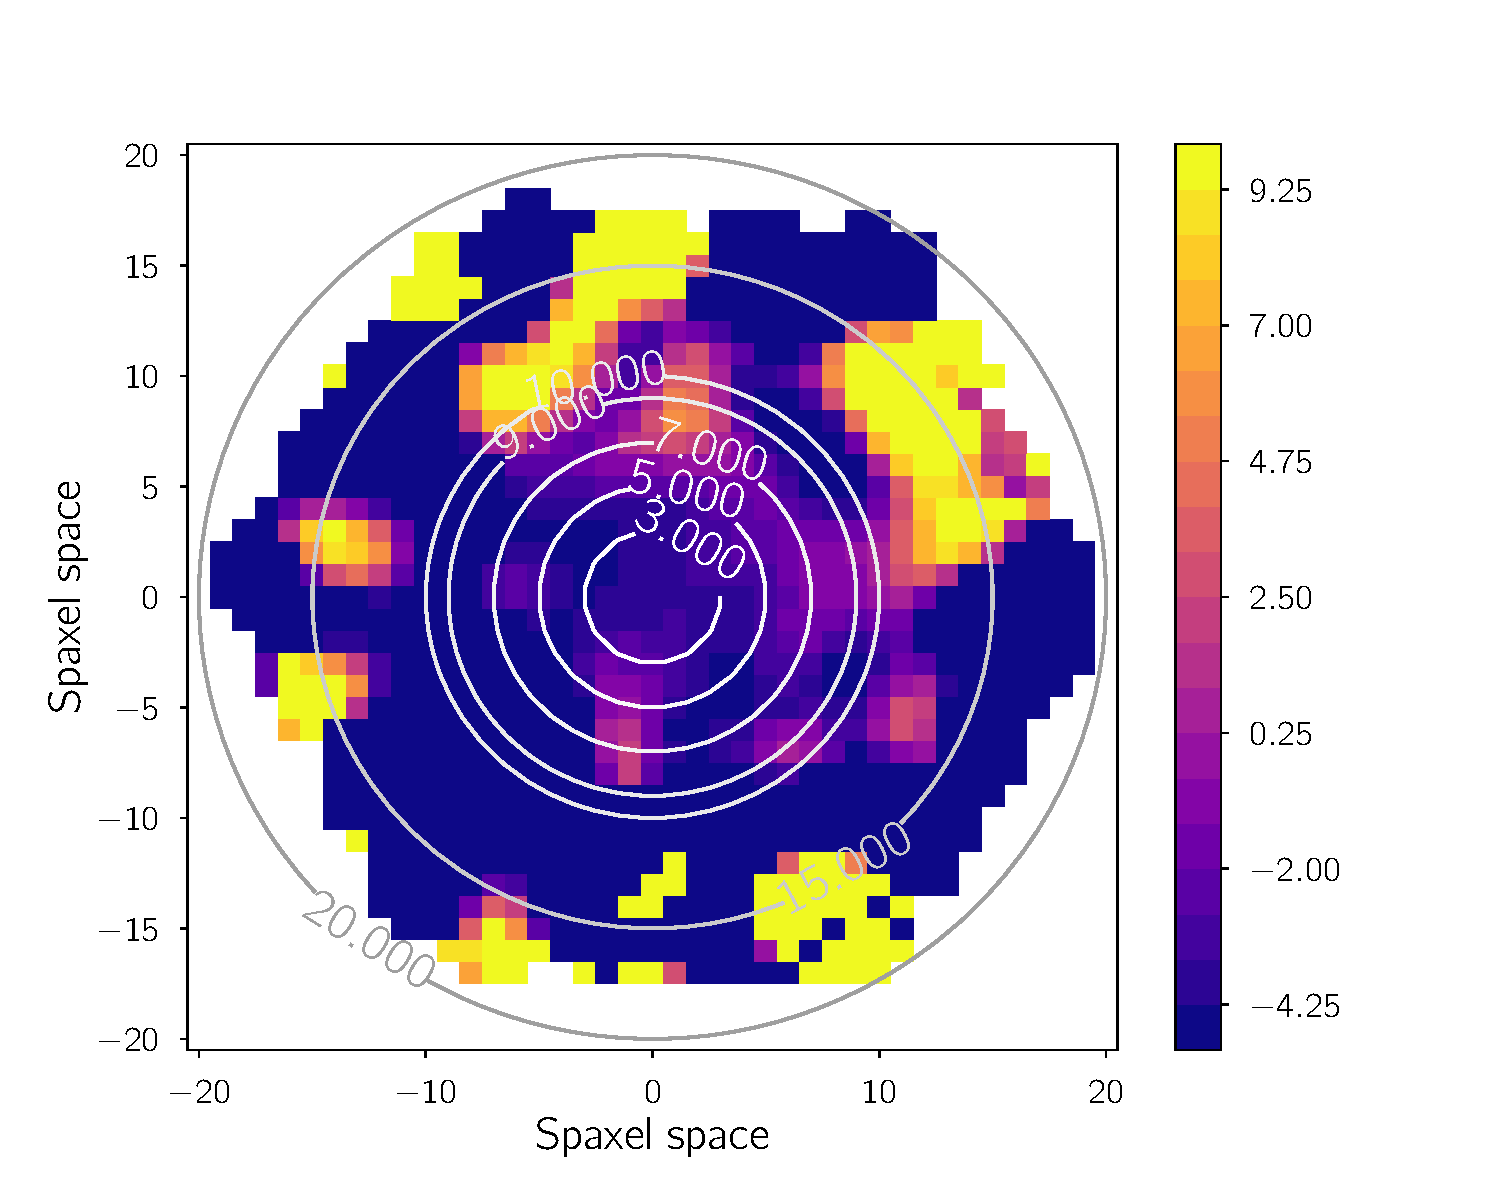
\includegraphics[width=\textwidth]{figures/gal_aperture.pdf}
%\caption[Placeholder figure: TBD. Sample MaNGA galaxy 
%view in the spaxel space with the $H{\delta_{\rm A}}$ distribution 
%plotted as a function of position and the contours marking 
%the aperture diameters at different angular distances in arcseconds]
%{Placeholder figure: TBD. Sample MaNGA galaxy view 
%in the spaxel space with the $H_{\delta_{\rm A}}$ distributions 
%plotted as a function of position and the contours 
%marking the aperture diameters at different angular distances in arcseconds
%\label{fig:sample_manga}}
%\end{figure}

For any MaNGA galaxy at redshift $z_{\rm obs}$, we can simulate what
the SDSS Main Sample spectrum would have looked like if it had observed the 
galaxy at that redshift or any higher redshift. We simply calculate the 
spectrum within an aperture that is 3$''$ diameter (if we are simulating 
the Main Sample spectrum at $z_{\rm obs}$) or larger (if we are simulating
the spectrum at a larger $z$).
The transverse angular distance varies with redshift as follows:
$$D_{\rm A}(z) = \frac{D_{\rm M}(z)}{1+z}, $$
where $D_{\rm M}(z)$ is the co-moving distance at redshift z.
So when a galaxy at $z_{\rm obs}$ is shifted to some other
$z_{\rm new}$ the new distance $d_{\rm new}$ of spaxel $(x,y)$ 
from the central spaxel $(x_{c},y_{c})$ relates to the old distance thus:
$$ d_{\rm new} = \frac{(1+z_{\rm new})\times D_{\rm M}(z_{\rm obs}) \times d}{(1+z_{\rm obs}) \times  D_{\rm M}(z_{\rm new})} $$
This equation allows us to define a new aperture of $d_{\rm new} < 3''$.

For any spectral measurement we can then compare the measurement
of the total spectrum in the MaNGA cube to that which would have been
measured through a 3$''$ aperture at a given redshift. Since galaxies
come in a range of sizes and spectral profiles, this difference
will vary from galaxy to galaxy and we must look at a large sample.
Importantly, for a chosen redshift $z_{\rm new}$ at which to evaluate
the degree of bias, we can only use a sample of galaxies with 
$z_{\rm obs} \le z_{\rm new}$.

\begin{figure}
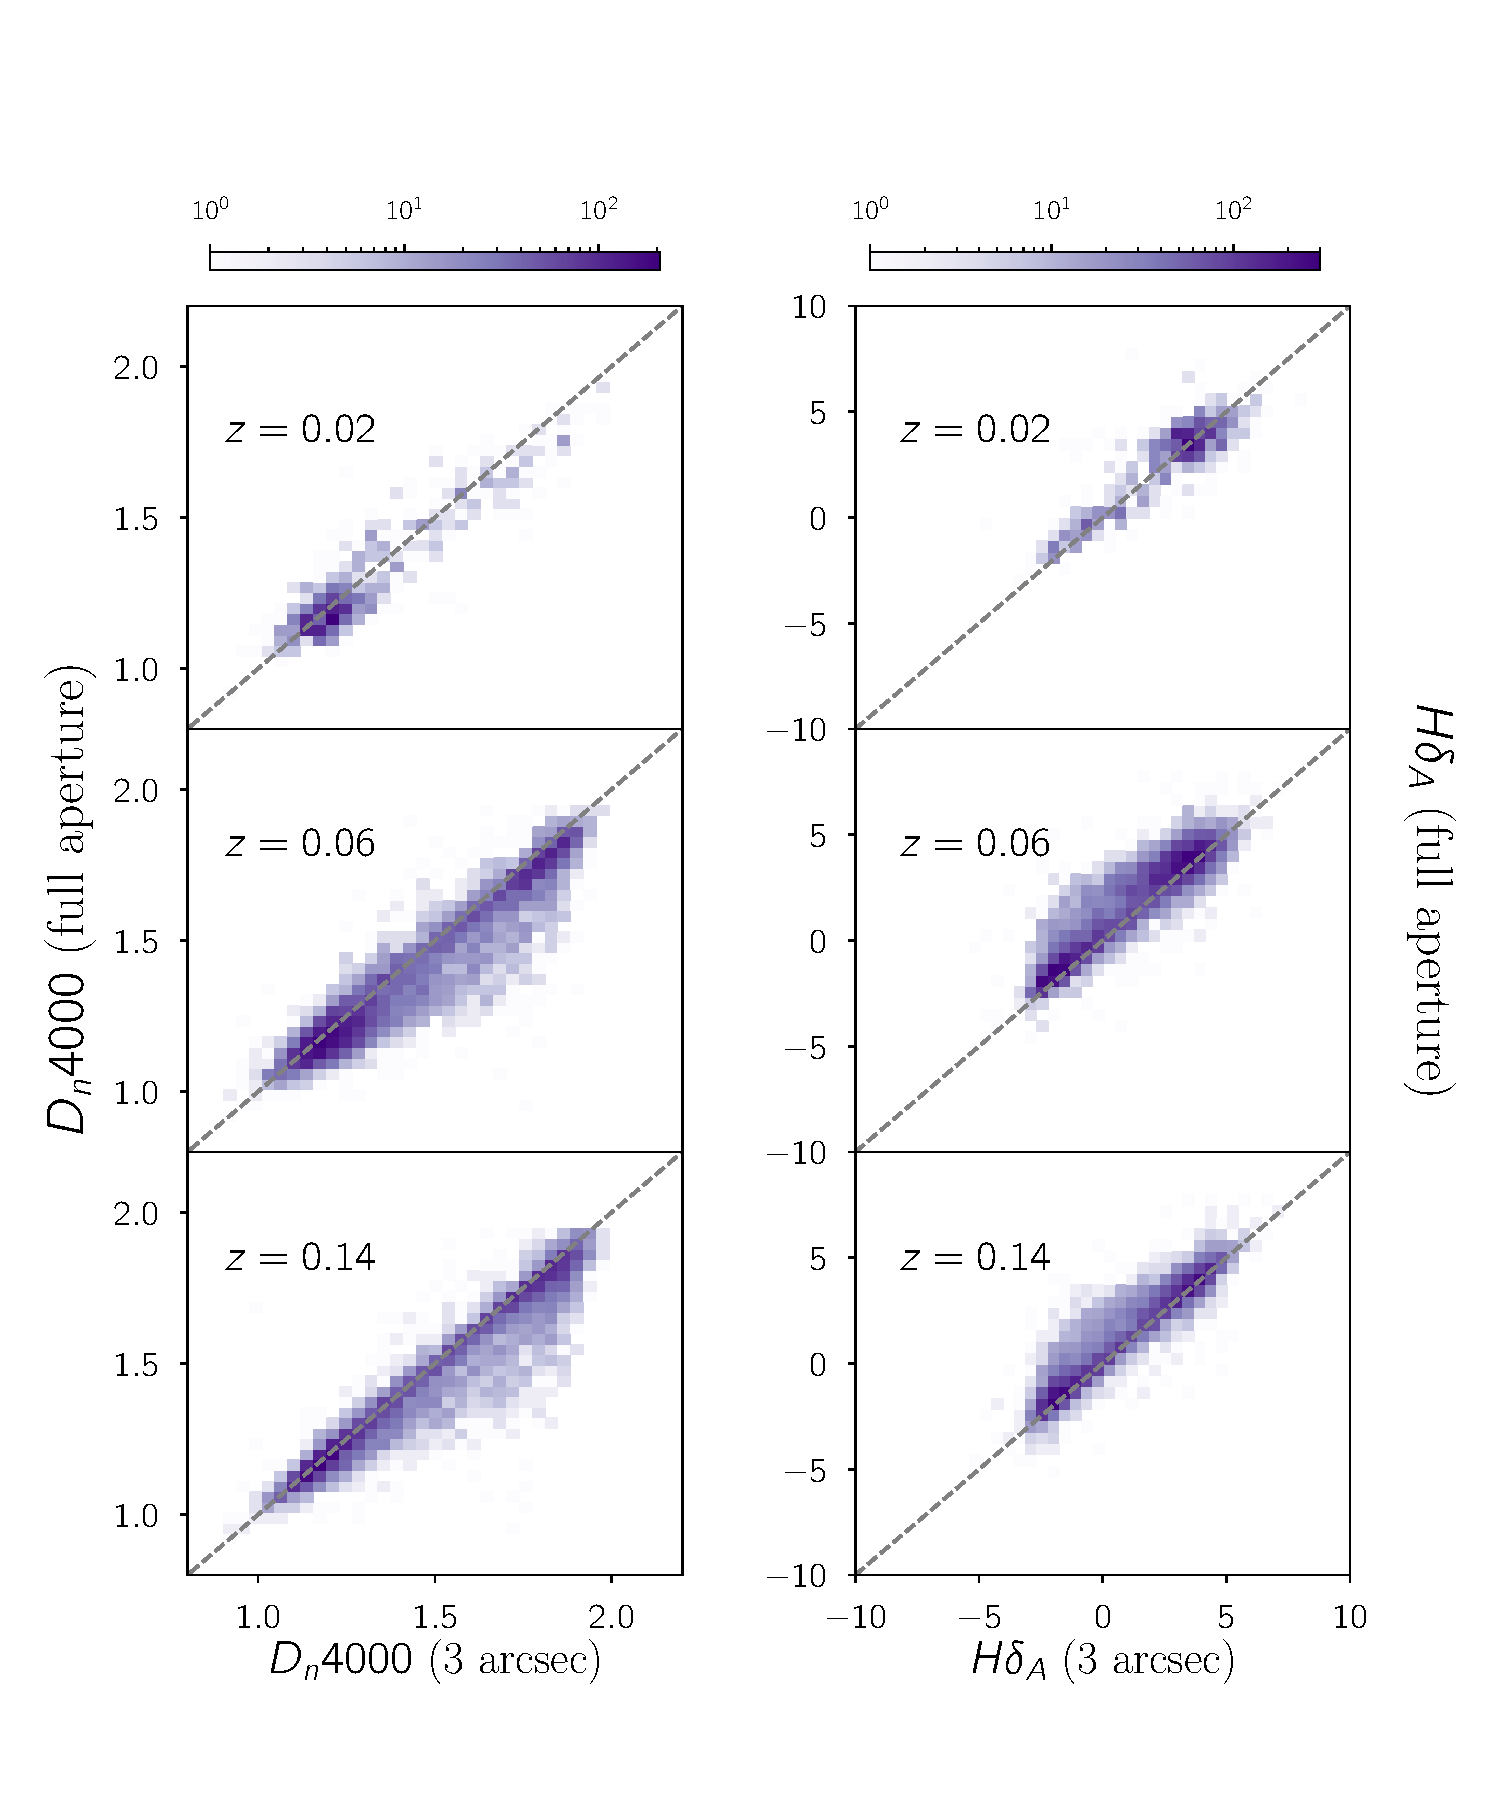
\includegraphics[width=\textwidth]{figures/full_aperture_comparisons.pdf}
\caption[The $D_{n}4000$, $h\delta_{A}$ indices measured at 
$z = 0.02,0.06,0.14$ with a $3''$ aperture compared to the full aperture measurement]
{ The $D_{n}4000$ and $H\delta_{A}$ indices measured 
at $z = 0.02,0.06,$ and $0.14$ with a $3''$ aperture 
compared to the full aperture measurement. The dashed line corresponds
to $x=y$.
\label{fig:redshift_comparison}}
\end{figure}


I measure $H\delta_{\rm A}$ and $D_{\rm n}4000$ indices in the standard
fashion in the galaxy rest frames. To perform the measurements more 
efficiently, for each spaxel I measure the $H\delta_{\rm A}$ central
and side bands and the two $D_{\rm n}4000$ bands, and store these five
numbers separately. Then, instead of needing to access and coadd the full
spectra, for each aperture I only need to add each of these five numbers
across the relevant spaxels. I then combine them into the two index
measurements following the procedure in Section 2.2.

\section{Results}
\subsection{Comparison to Full Aperture Measurements}

To investigate how the full aperture measurements compare to the 3$''$ 
measurements, I choose 3 different redshift bins $z = 0.02$, $0.06$, 
and $0.14$, and determine how offset the $H\delta_{\rm A}$ and 
$D_{\rm n}4000$ measures are. For each redshift $z$, I pick the galaxies 
with redshifts $z_{\rm obs} < z$, ``shift" them to the cutoff 
redshift as described in Section \ref{sec:chap2methods}, 
and compare the full aperture measurements to the 3$''$
measurements that would be made at redshift $z$. 

The results of this procedure are shown in 
Fig. \ref{fig:redshift_comparison}, where the full 
aperture measurements are plotted against the 3$''$ measurements at 
the each redshift, with the colorbars indicating the number of galaxies 
in each bin. We note that the total number of galaxies at each redshift 
is 561 for $z = 0.02$, 5016 for $z = 0.06$ and 6402 for $z = 0.14$.\\

We first note the systematic change in the MaNGA sample between $z\sim 0.02$
and $z\sim 0.14$, which is related to MaNGA's target selection procedure. 
In order to achieve the desired areal coverage, MaNGA's selection
of galaxies is such that the lower redshift galaxies are lower luminosity
and mass. These lower luminosity galaxies are more star forming and have
older stellar populations, so they have deeper $H\delta_{A}$ and weaker 
$D_{\rm n} 4000$. This trend is apparent in the variation in the galaxy
population from panel to panel. This trend means we need to look at all
of the panels to understand the comparison between $3''$ aperture and full
aperture measurements of these quantities.

\begin{figure}
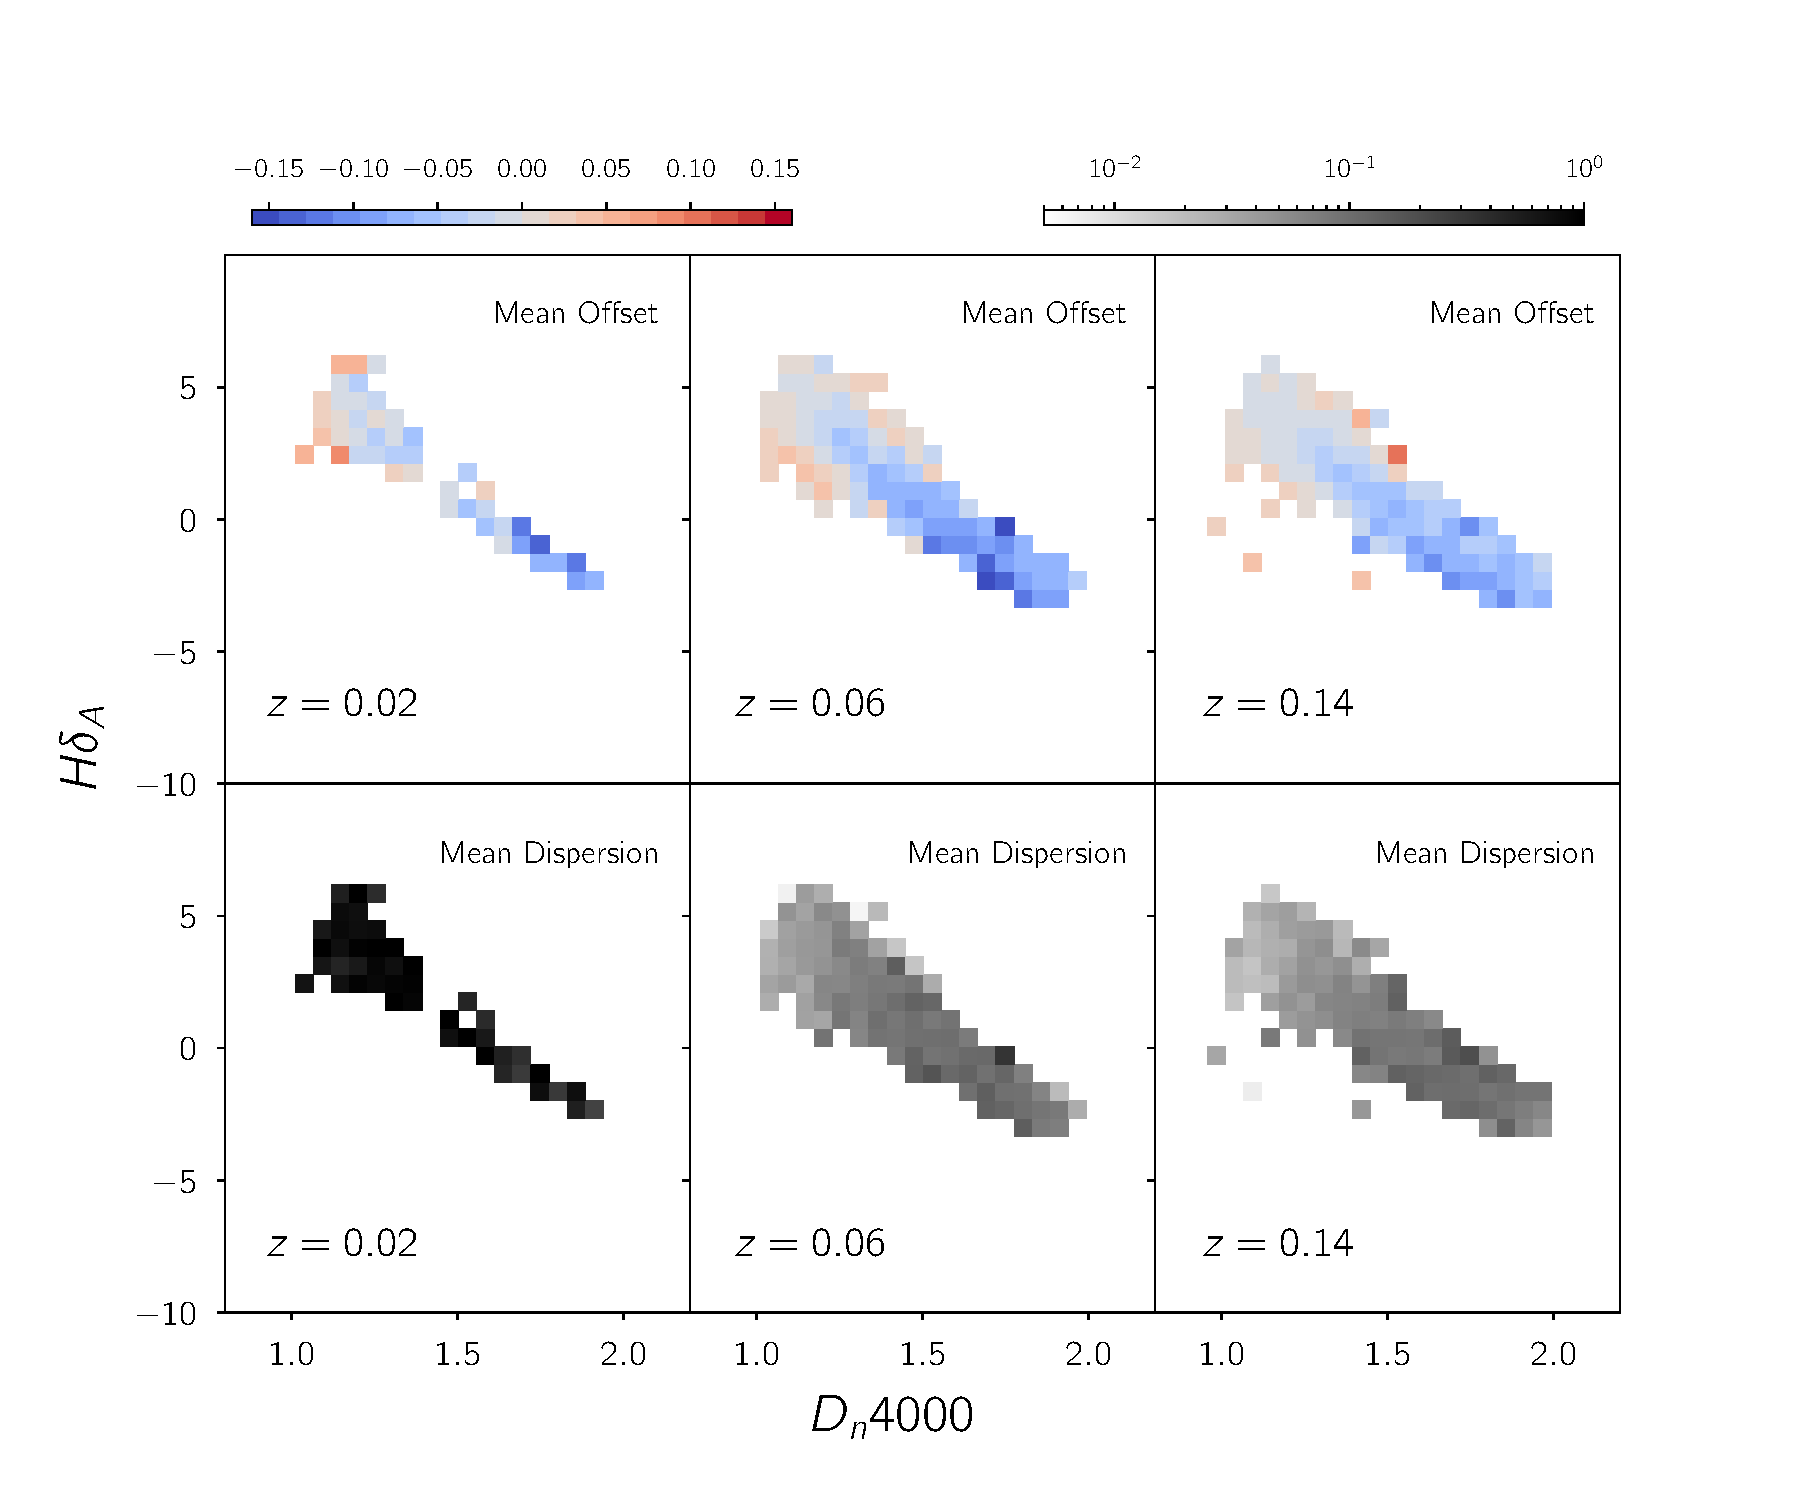
\includegraphics[width=\textwidth]{figures/dn4000_full_aperture_comparisons.pdf}
\caption[The mean offset and dispersion in the $D_{n}4000$ index measured 
at $z = 0.02,0.06$ and $0.14$ with a $3''$ aperture from the full aperture measurement]{ The mean offset and dispersion in the $D_{n}4000$ index measured at $z = 0.02,0.06$ and $0.14$ with a $3''$ aperture from the full aperture measurement
\label{fig:offset_d4000}}
\end{figure}

\begin{figure}
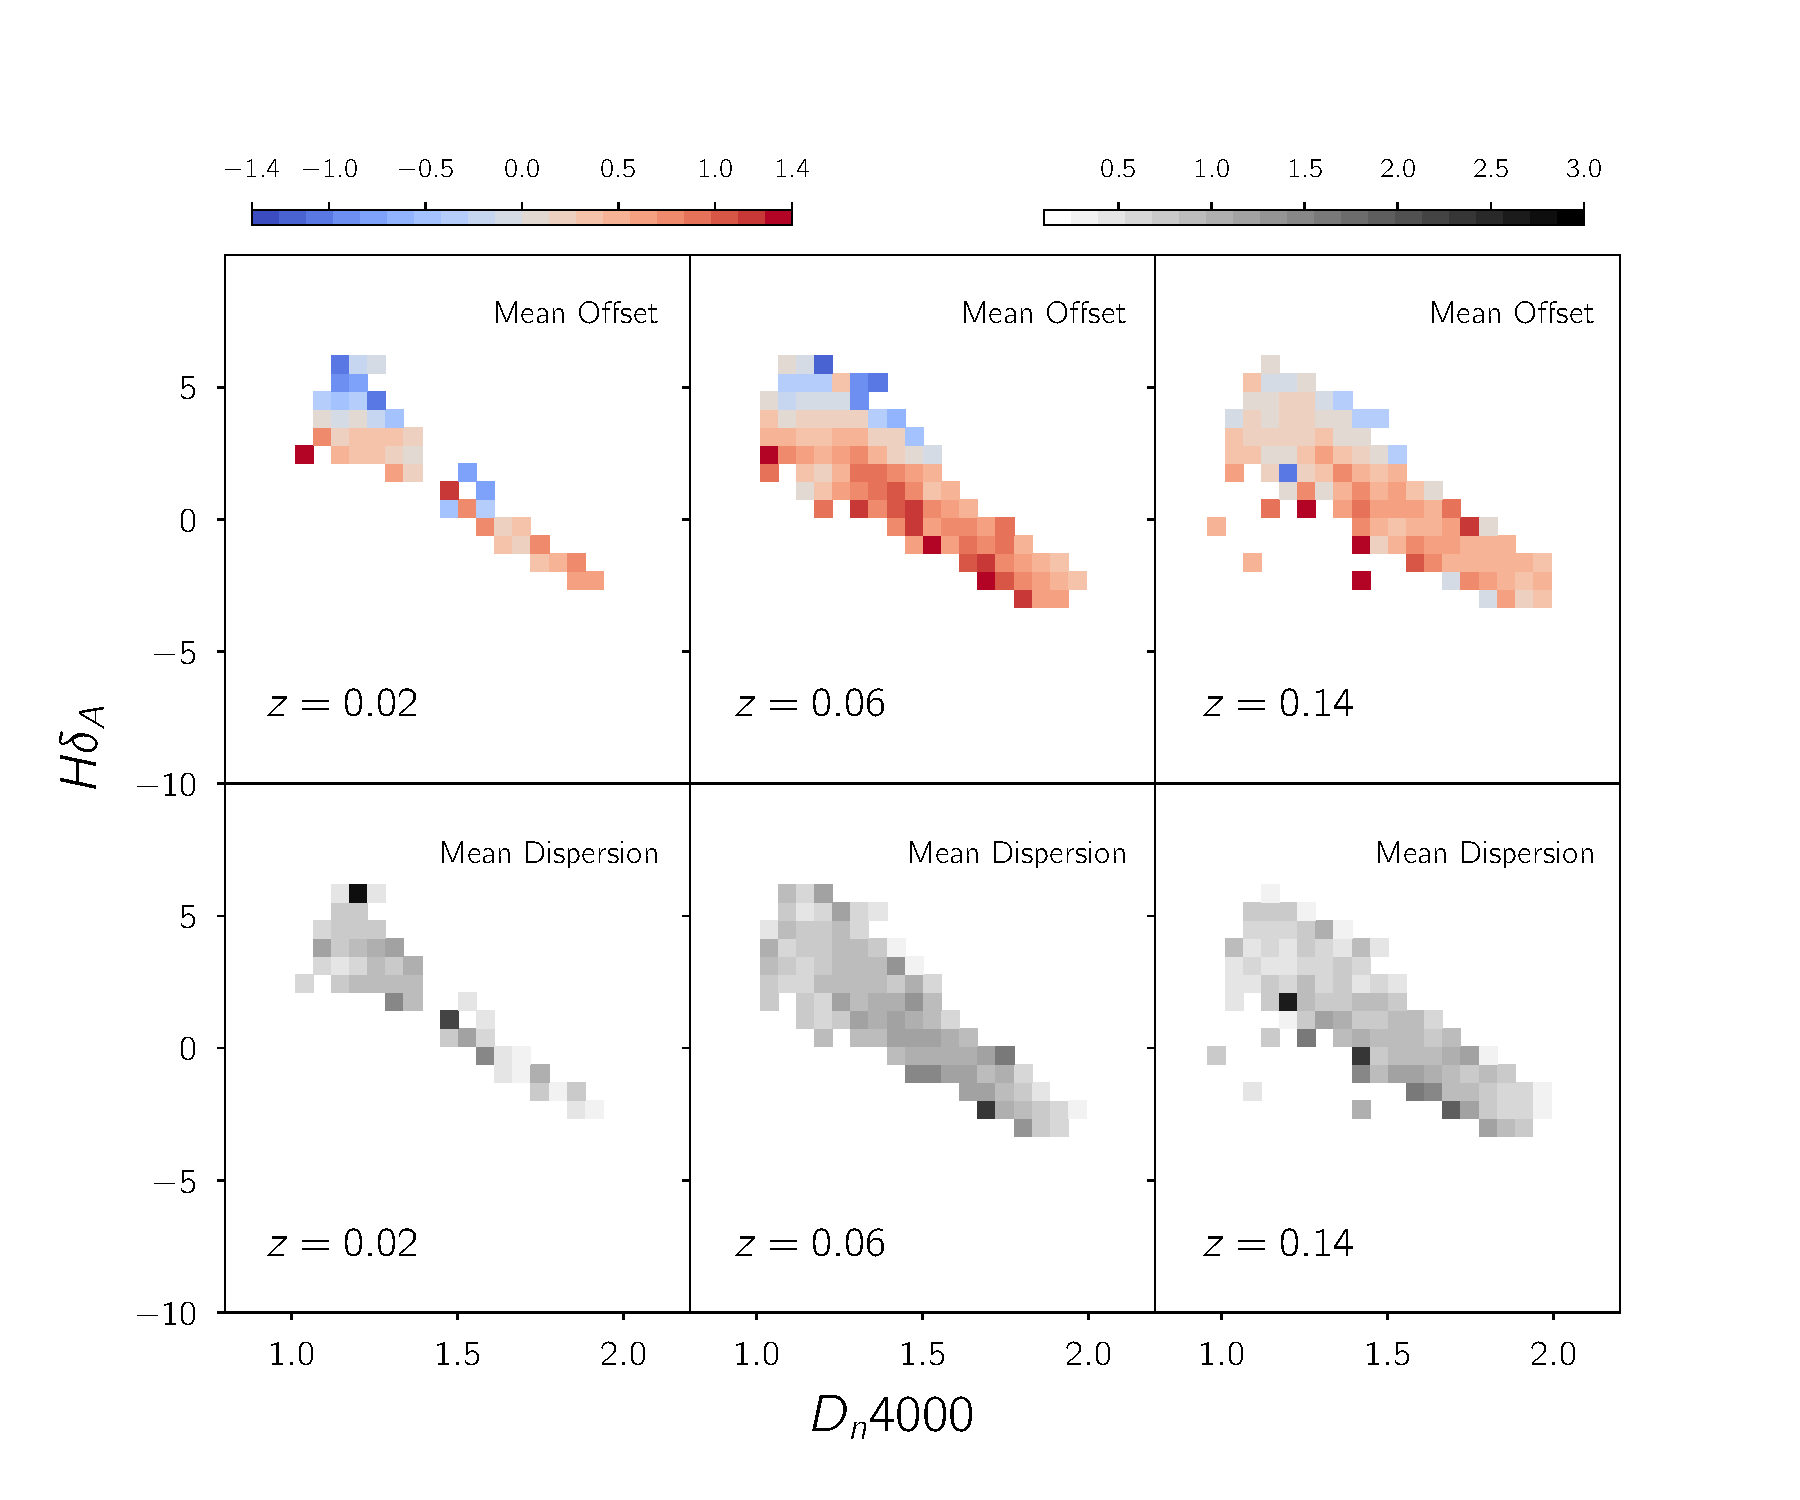
\includegraphics[width=\textwidth]{figures/hdelta_full_aperture_comparisons.pdf}
\caption[The mean offset and dispersion in the $H\delta_{A}$
 index measured at $z = 0.02,0.06$ and $0.14$ with a $3''$ 
 aperture from the full aperture measurement ]
 {The mean offset and dispersion in the $H\delta_{A}$ 
 index measured at $z = 0.02,0.06$ and $0.14$ 
 with a $3''$ aperture from the full aperture measurement.
\label{fig:offset_hdelta}}
\end{figure}

From Fig. \ref{fig:redshift_comparison}, we can infer the following. For 
many galaxies the offset is pretty minimal; they fall pretty close 
to the $x=y$ line. The scatter is largest at $z = 0.06$, and this scatter
tends towards higher $D_{\rm n}4000$ and lower $H\delta_{\rm A}$ values 
relative to the full aperture measurements, particularly for galaxies with
intermediate $D_{\rm n}4000$ and $H\delta_{\rm A}$ values for the full
aperture. This effect is likely due to spiral galaxies with strong galactic
bulges. These galaxies are common at the masses populating the $z_{\rm obs} < 0.06$
bin, and have the property that their bulges are considerably less star-forming
than their disks. Thus, the 3$''$ aperture might cover their bulge but not their
disk, and therefore show higher $D_{\rm n} 4000$ and lower $H\delta_{A}$
than the full aperture measurement. This effect is less prominent 
at $z=0.02$ because the galaxies in the MaNGA sample at those redshifts 
are lower luminosity and 
have less prominent bulges. The scatter also lessens as we approach $z = 0.14$, 
close to the survey limit; although this sample also contains spirals with
strong bulges,  the 3$''$ aperture is larger with respect to the total size
of galaxies at this redshift.\\

From this figure, we conclude generally that the restrictions of
how the MaNGA sample is selected make it hard to evaluate the effects 
of the aperture bias at the lowest redshifts ($z\sim 0.02$) --- 
clearly the sample there is not representative of the sample as a whole.
However, the $z=0.06$ and $z=0.14$ cases bracket the median redshift of the 
SDSS Main Sample so will characterize the aperture bias well for much
of that sample. We can guess already that the general effect will be that
the $3''$ fiber will overestimate the stellar ages and therefore their 
mass-to-light ratios, for some fraction of the galaxies.

\begin{figure}
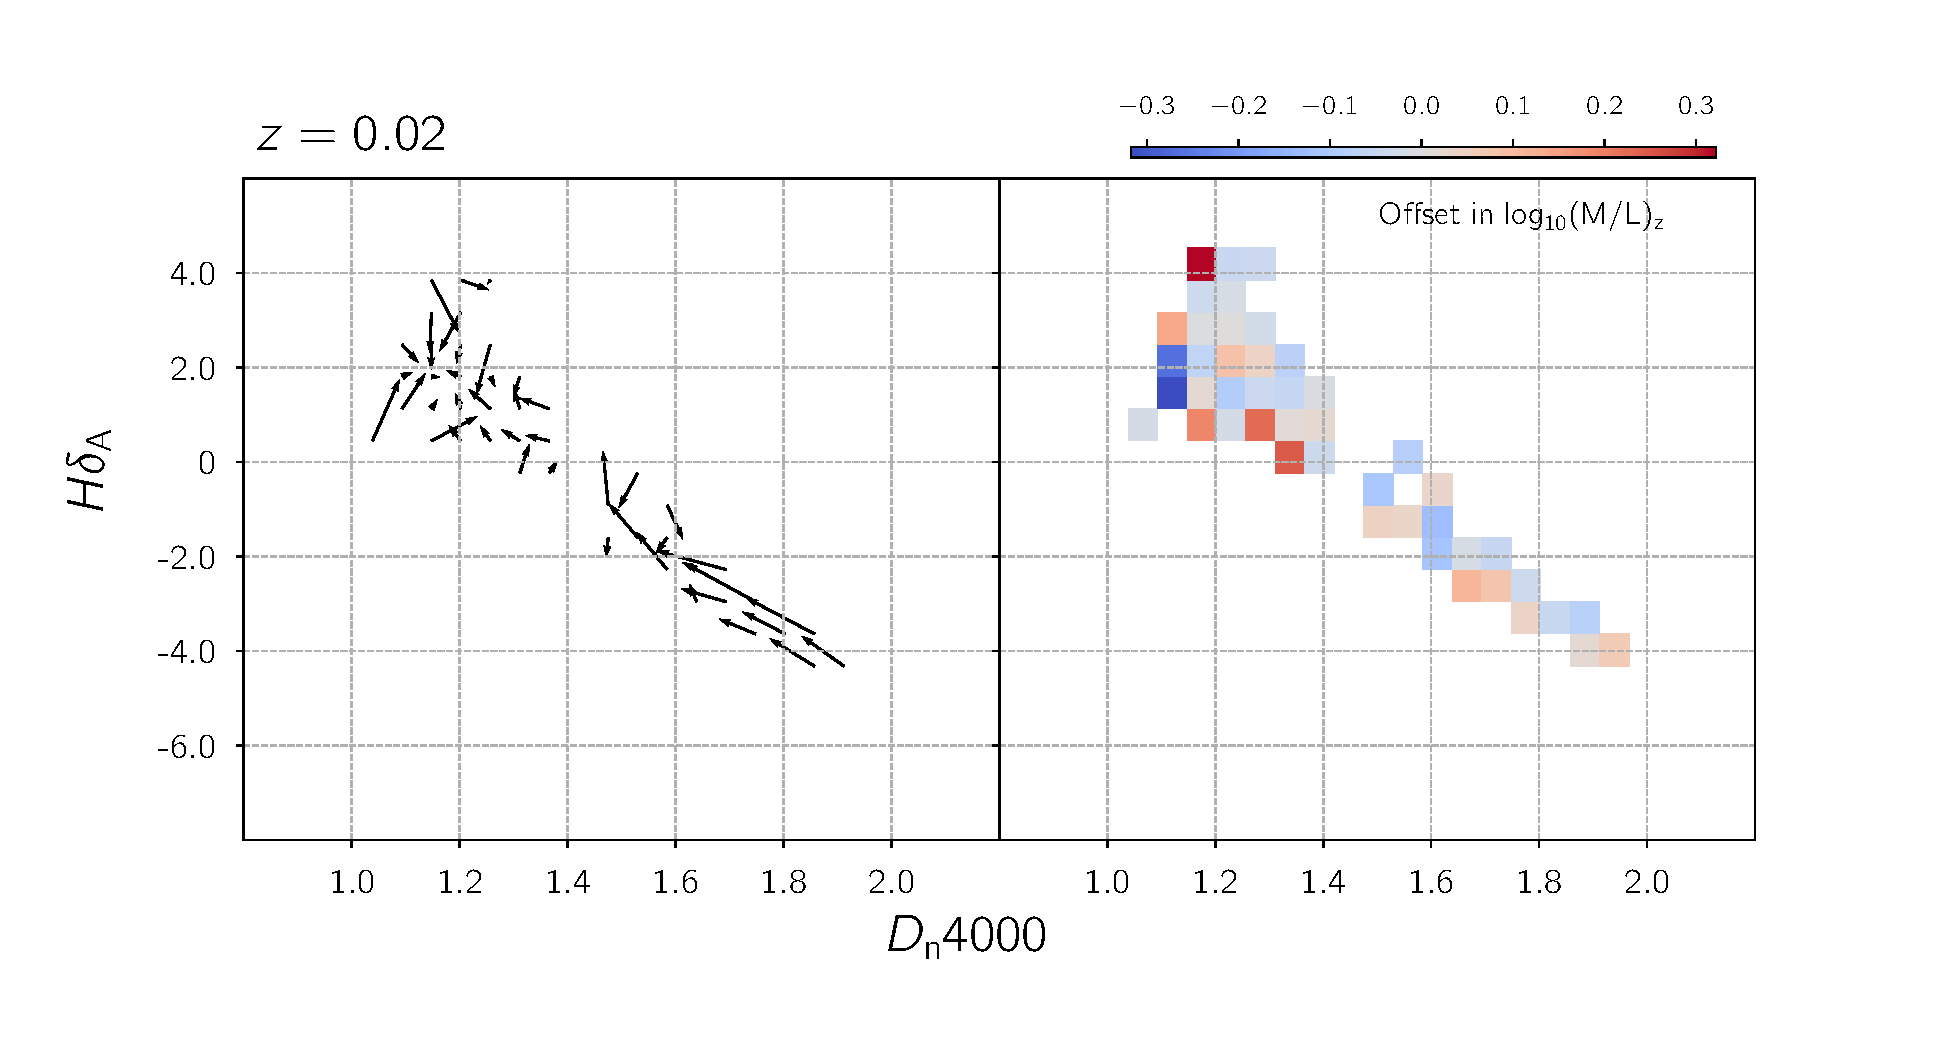
\includegraphics[width=\textwidth]{figures/mlz_offset_a.pdf}
\caption[  \emph{Left:} The combined mean offset in 
$D_{\rm n}4000$-$h\delta_{\rm A}$ at $z=0.02$ from the full aperture 
measurements, represented as a vector whose projections on the axes 
are the actual offsets in either direction. 
\emph{Right:} The offsets transformed to the $z$-band mass-to-light ratios 
using the grid in Figure \ref{fig:kauff_grid}. ]{ \emph{Left:} The combined 
mean offset in $D_{\rm n}4000$-$h\delta_{\rm A}$ at $z=0.02$ from 
the full aperture measurements represented as a vector whose projections 
on the axes are the actual offsets in either direction. 
\emph{Right:} The offsets transformed to the $z$-band mass-to-light 
ratios using the grid in Figure \ref{fig:kauff_grid}.
\label{fig:offset_quiver1}}
\end{figure}

\begin{figure}
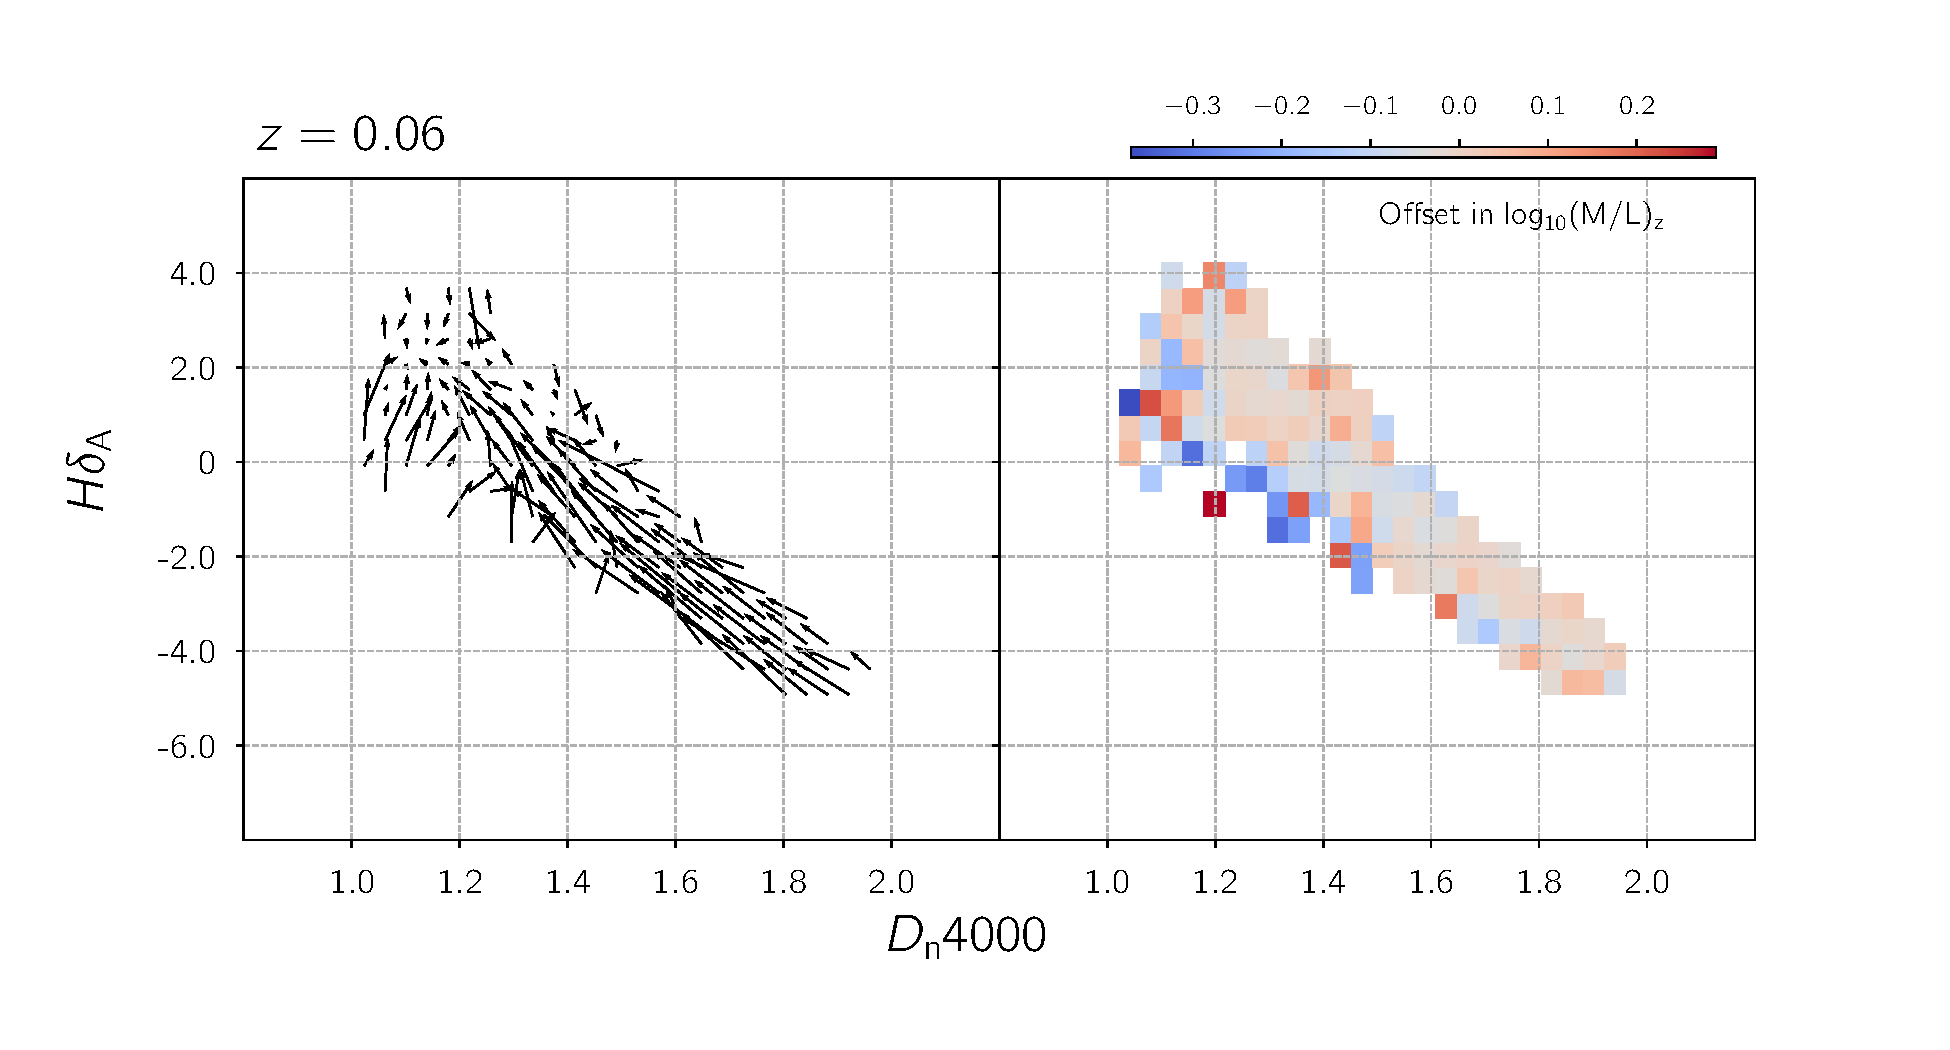
\includegraphics[width=\textwidth]{figures/mlz_offset_b.pdf}
\caption[  \emph{Left:} The combined mean offset in $D_{\rm n}4000$-$h\delta_{\rm A}$ at $z=0.02$ from the full aperture measurements represented as a vector whose projections on the axes are the actual offsets in either direction. \emph{Right:} The offsets transformed to the z-band mass-to-light ratios using the grid in Figure \ref{fig:kauff_grid}. ]{ \emph{Left:} The combined mean offset in $D_{\rm n}4000$-$h\delta_{\rm A}$ at $z=0.06$ from the full aperture measurements represented as a vector whose projections on the axes are the actual offsets in either direction. \emph{Right:} The offsets transformed to the z-band mass-to-light ratios using the grid in Figure \ref{fig:kauff_grid}.
\label{fig:offset_quiver2}}
\end{figure}


\subsection{Offsets in the $H\delta_{\rm A}$-$D_{\rm n}4000$ plane}

\begin{figure}
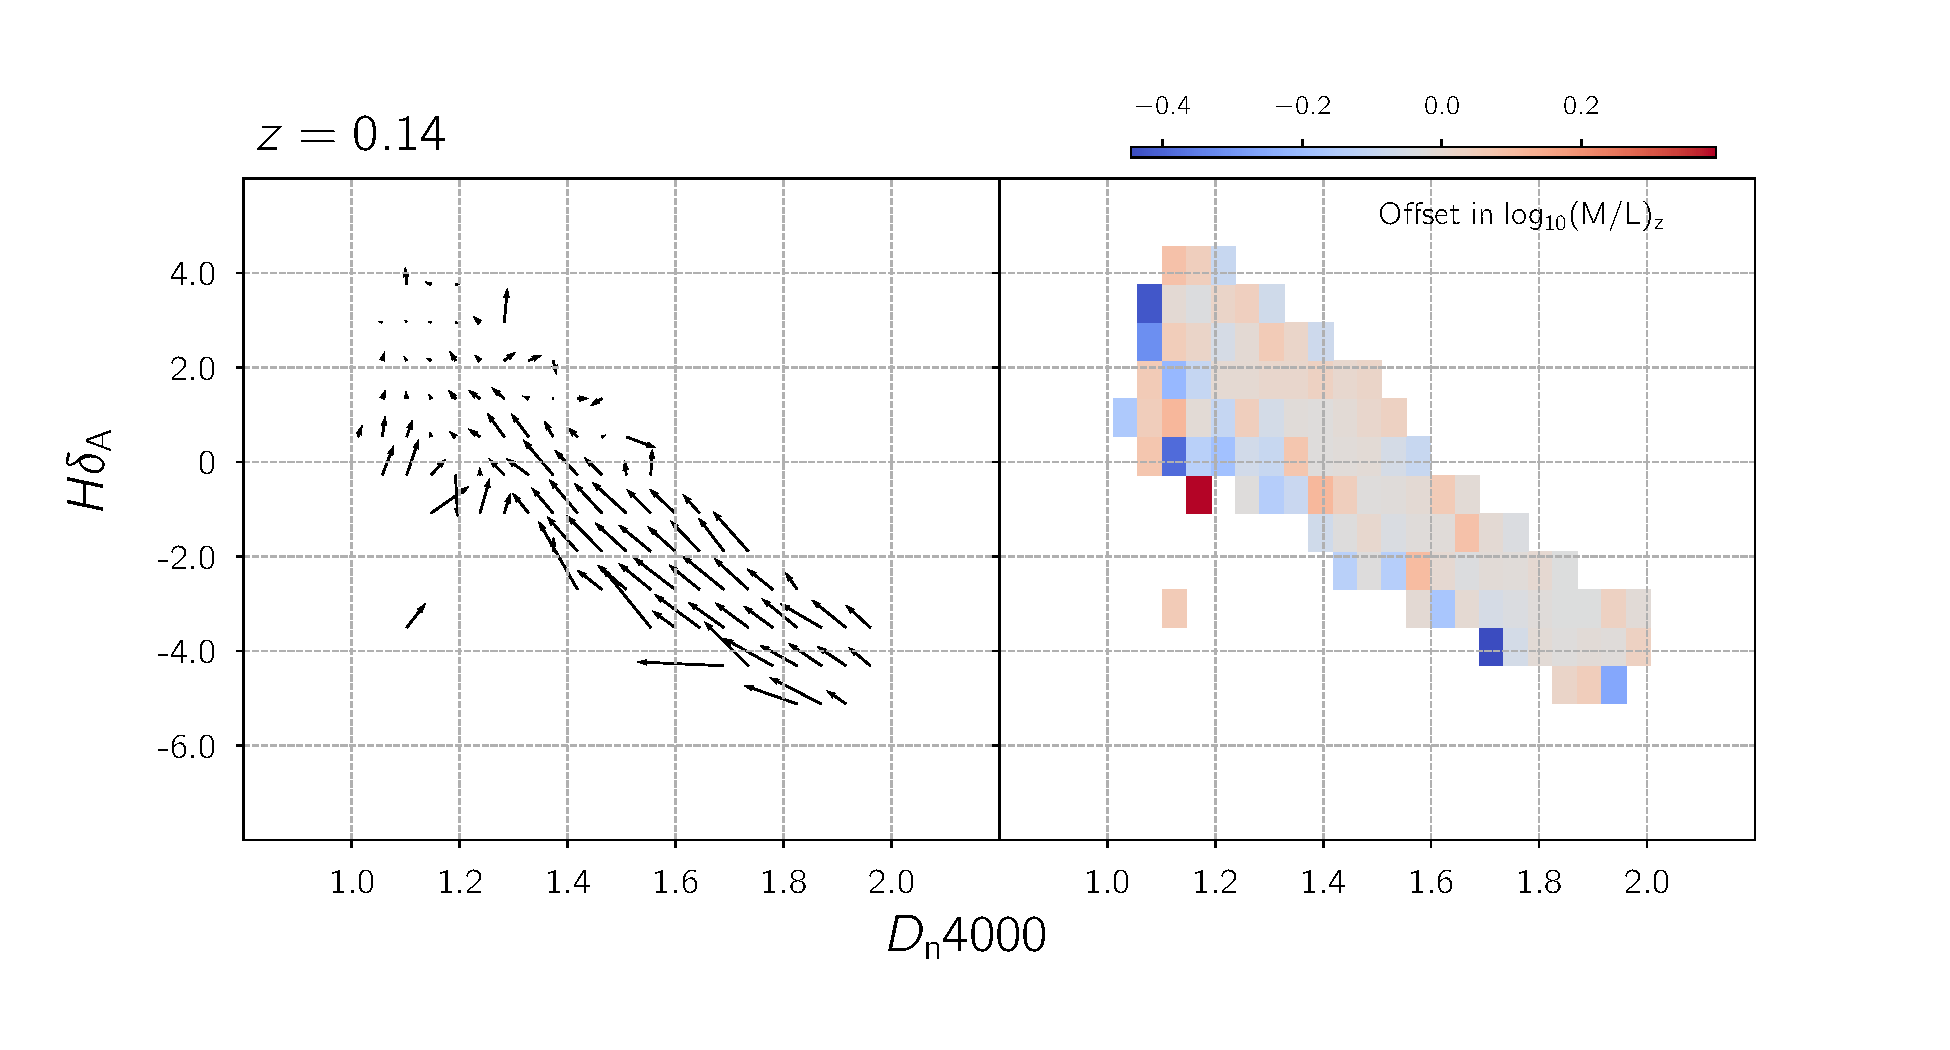
\includegraphics[width=\textwidth]{figures/mlz_offset_c.pdf}
\caption[ \emph{Left:} The combined mean offset in $D_{\rm n}4000$-$h\delta_{\rm A}$ at $z=0.14$ from the full aperture measurements represented as a vector whose projections on the axes are the actual offsets in either direction. \emph{Right:} The offsets transformed to the z-band mass-to-light ratios using the grid in Figure \ref{fig:kauff_grid}. ]{ \emph{Left:} The combined mean offset in $D_{\rm n}4000$-$h\delta_{\rm A}$ at $z=0.14$ from the full aperture measurements represented as a vector whose projections on the axes are the actual offsets in either direction. \emph{Right:} The offsets transformed to the z-band mass-to-light ratios using the grid in Figure \ref{fig:kauff_grid}.
\label{fig:offset_quiver3}}
\end{figure}

The next step in comparing the full aperture measurements to the 3$''$
measurements is to determine where the galaxies move in the 
H$\delta_{\rm A}$ - $D_{\rm n}4000$ plane for each of the redshift 
bins. We bin the galaxies according to the 3$''$ measurements
in both $D_{\rm n}4000$ and H$\delta_{\rm A}$, and measure the 
mean and standard deviation within each bin of the offsets between
the 3$''$ and full aperture measurements. Figure \ref{fig:offset_d4000} 
shows the mean offsets and standard deviations for the 
$D_{\rm n}4000$ measurements. Figure 
\ref{fig:offset_hdelta} shows the mean offsets and standard deviations
for the  H$\delta_{\rm A}$ measurements. 
The general tendency we see in the $D_{\rm n}4000$ offsets is that 
the older galaxies tend to have slightly negative offsets and the 
younger ones tend to have slightly positive offsets. In the case of 
H$\delta_{\rm A}$, the offsets on average tend to be mostly positive 
(in this case, tending toward the region of phase space with 
younger galaxies) with the exception of a few bins with high 
H$\delta_{\rm A}$ where there are a few small negative offsets.\\

\begin{figure}
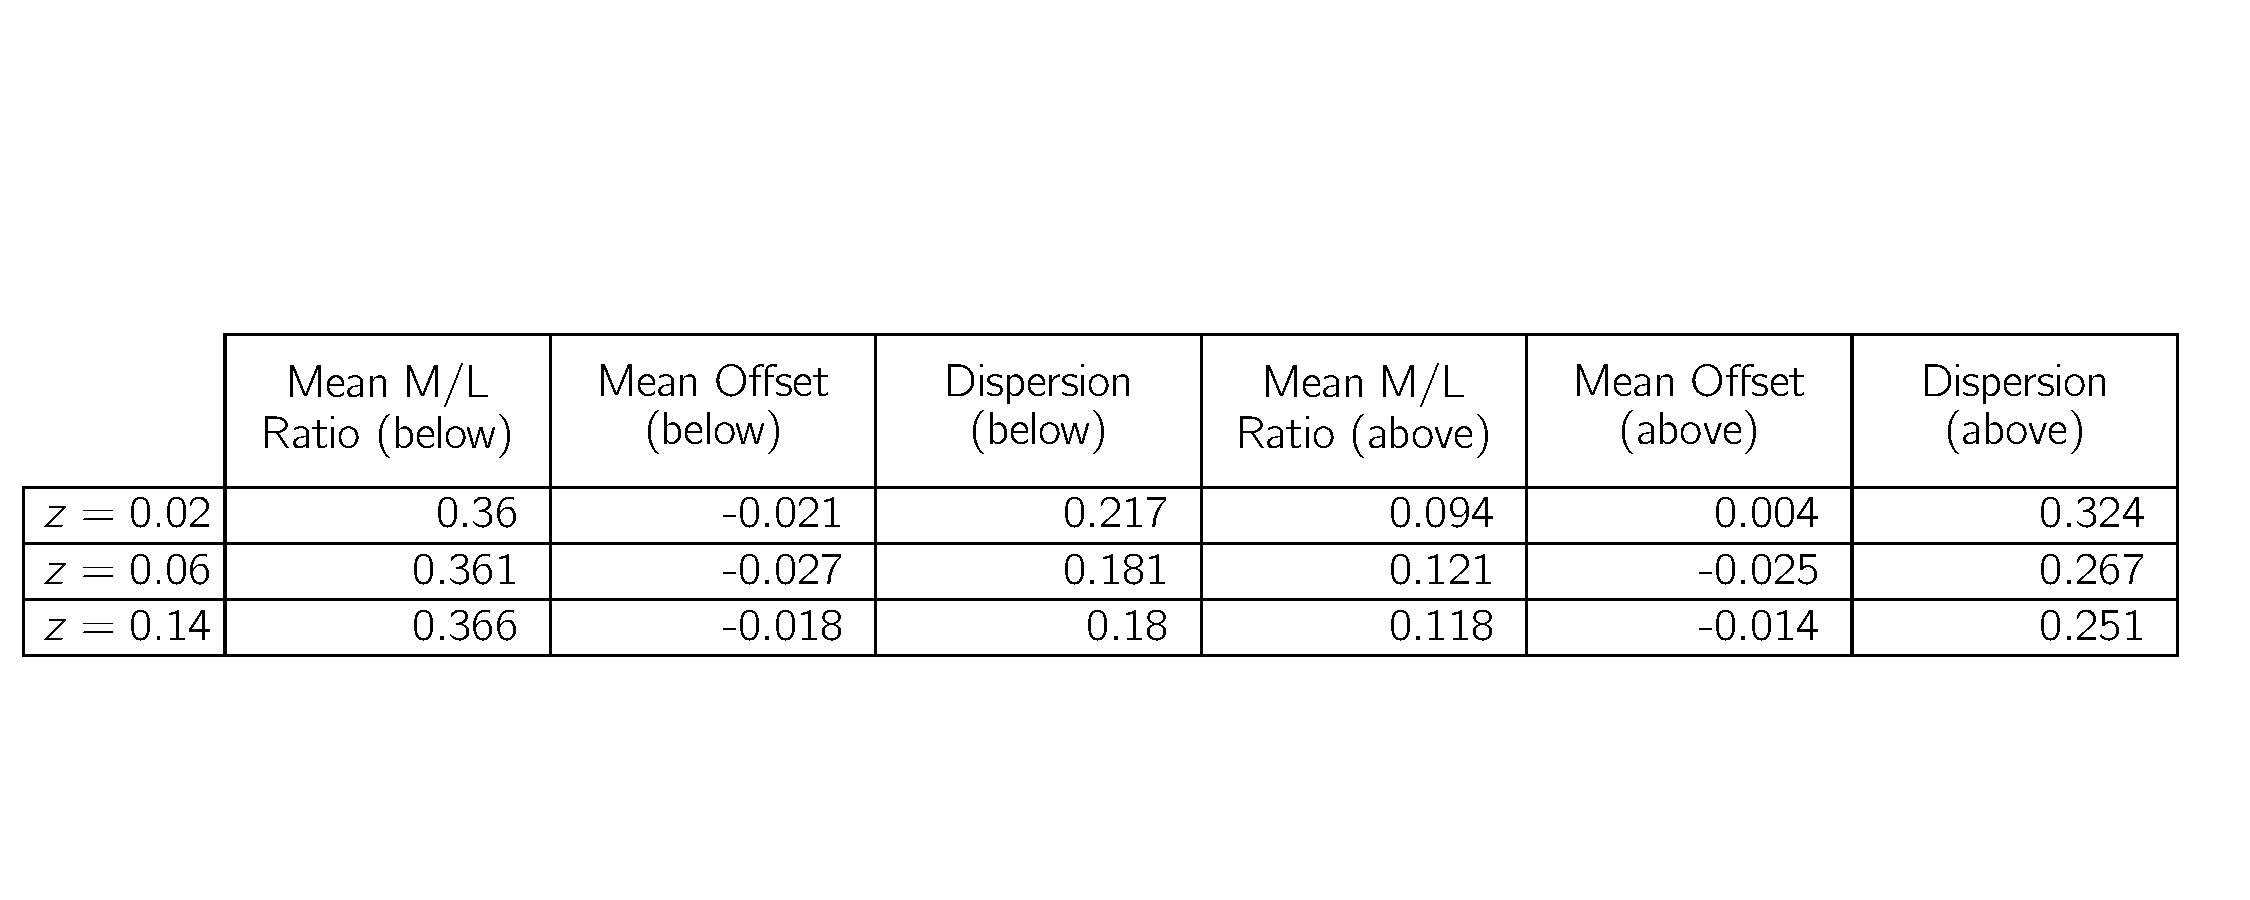
\includegraphics[width=\textwidth]{figures/table.pdf}
\caption[Table showing the mean offsets for the three redshift bins.]
{Table showing the mean offsets for the three redshift bins
\label{tab: mean_offset_table}}
\end{figure}

The combined offsets in both the directions are plotted as quiver 
plots that occupy the left subplots in Figures \ref{fig:offset_quiver1}, 
\ref{fig:offset_quiver2} and \ref{fig:offset_quiver3}. The length of 
the vector offsets in the quiver plots can translate into very 
different offsets in ${\rm log}_{10}((M/L)_{z})$ depending on 
where they occur in the H$\delta_{\rm A}$ - $D_{\rm n}4000$ plane. 
Using the MPA-JHU mass-to-light ratios and index measurements 
for SDSS DR8 galaxies, we have reconstructed the transformation 
from a ($D_{\rm n}4000$, H$\delta_{\rm A}$) value to a 
${\rm log}_{10}((M/L)_{z})$ value by interpolating the grid 
shown in Figure \ref{fig:kauff_grid}. Thus each offset in the 
plane can be converted to an offset in terms of the 
mass-to-light ratios. These mass-to-light ratio offsets are 
plotted in the right subplots in the aforementioned figures.\\ 
\begin{figure}
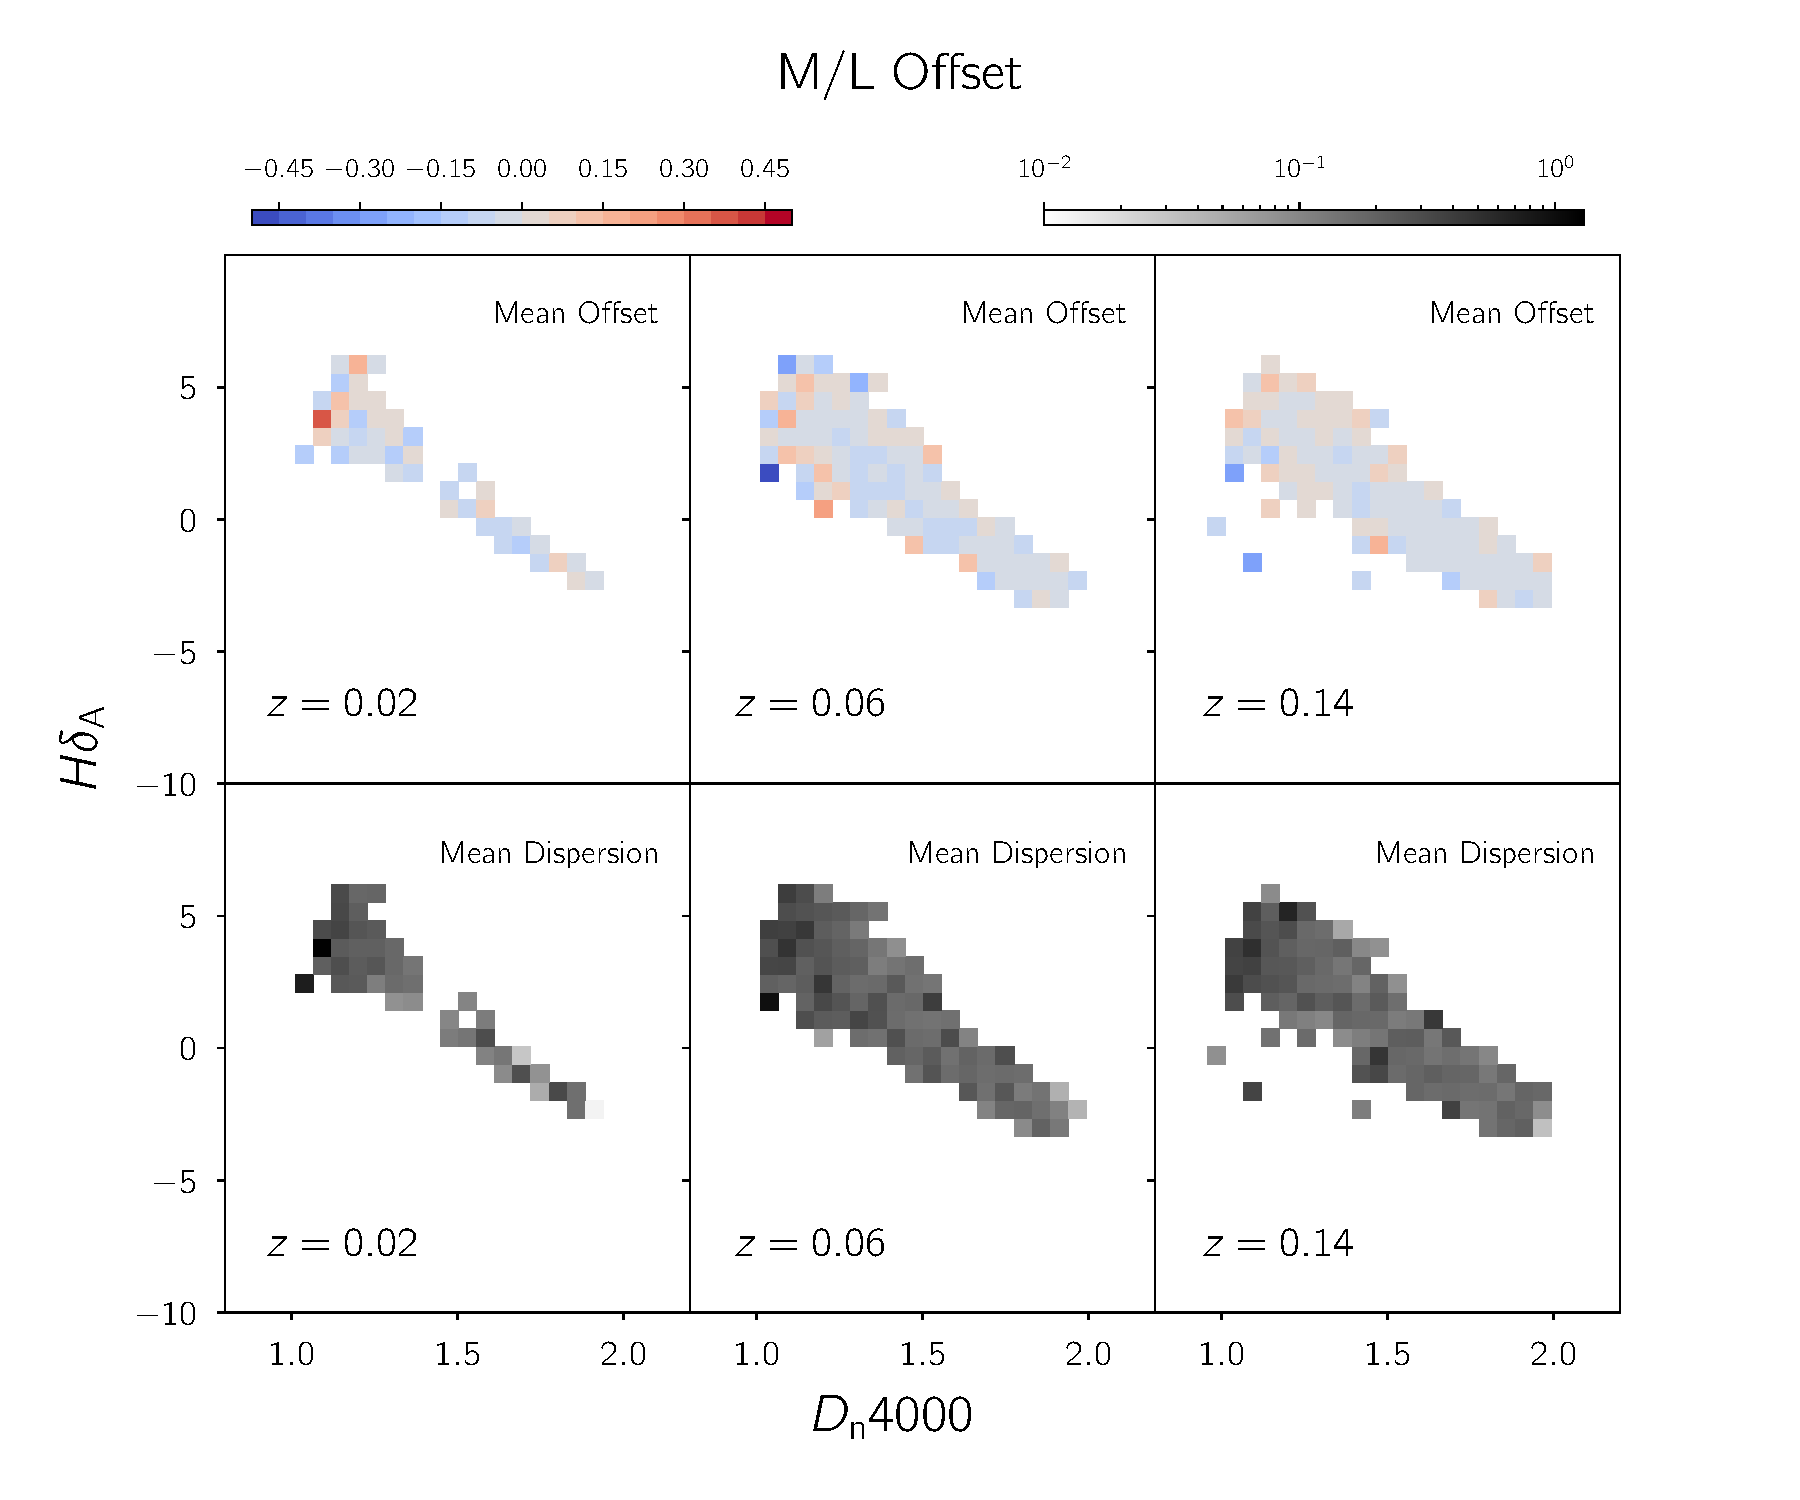
\includegraphics[width=\textwidth]{figures/ml_offset_plot.pdf}
\caption[ The mean and dispersion of the mass-to-light ratio 
offsets in each of the redshift bins binned along the $D_{\rm n}4000$ 
and H$\delta_{\rm A}$ axes. It is evident that the mean offsets for 
all galaxies are relatively small while the scatter about the mean
is significant relative to the mean.]{The mean and dispersion of the mass-to-light ratio 
offsets in each of the redshift bins binned along the $D_{\rm n}4000$ 
and H$\delta_{\rm A}$ axes. It is evident that the mean offsets for 
all galaxies are relatively small while the scatter about the mean
is significant relative to the mean.
\label{dispersion_plot}}
\end{figure}

Figure \ref{dispersion_plot} summarizes these findings, showing
the mass-to-light ratio offset and standard deviation in each bin 
for each redshift.
We quantity these findings in Tables \ref{tab: mean_offset_table} 
and  \ref{tab: median_offsets}. For these tables, we evaluate the
mean and median offsets and the standard deviations for the older 
and younger galaxies, separated using the cut in the 
$D_{\rm n}4000$-H$\delta_{\rm A}$ plane shown in 
Figure \ref{fig:kauff_grid}.  Table \ref{tab: median_offsets} also 
gives the median absolute deviation; these median absolute deviations
are smaller (by about 50\%) than would be expected for a Gaussian 
distribution given the standard deviations, indicating that the 
distributions have a somewhat longer tail to extreme values than
Gaussian.
 

\section{Discussion}
\label{ch2_discussion}
The results above lead us to the following conclusions:

\begin{itemize}
\item{The mean mass-to-light ratio offset for all galaxies is relatively 
small. Both Table \ref{tab: mean_offset_table} and Figure 
\ref{dispersion_plot} show that for both the younger and older galaxies 
in all bins, there is a slight negative mean and median offset.}
\item{The scatter about the mean is substantial relative to the mean. 
For the mid-redshift bin, the standard deviation for the older galaxies 
is $\sim 0.181$ and for the younger galaxies is $\sim 0.267$. These 
relatively large standard deviations imply that for individual galaxies, 
the effect of aperture bias large even if the average trend is small. 
This is also reflected in the uniformly high dispersions across bins 
in Figure \ref{dispersion_plot}.}
\end{itemize}

\begin{figure}
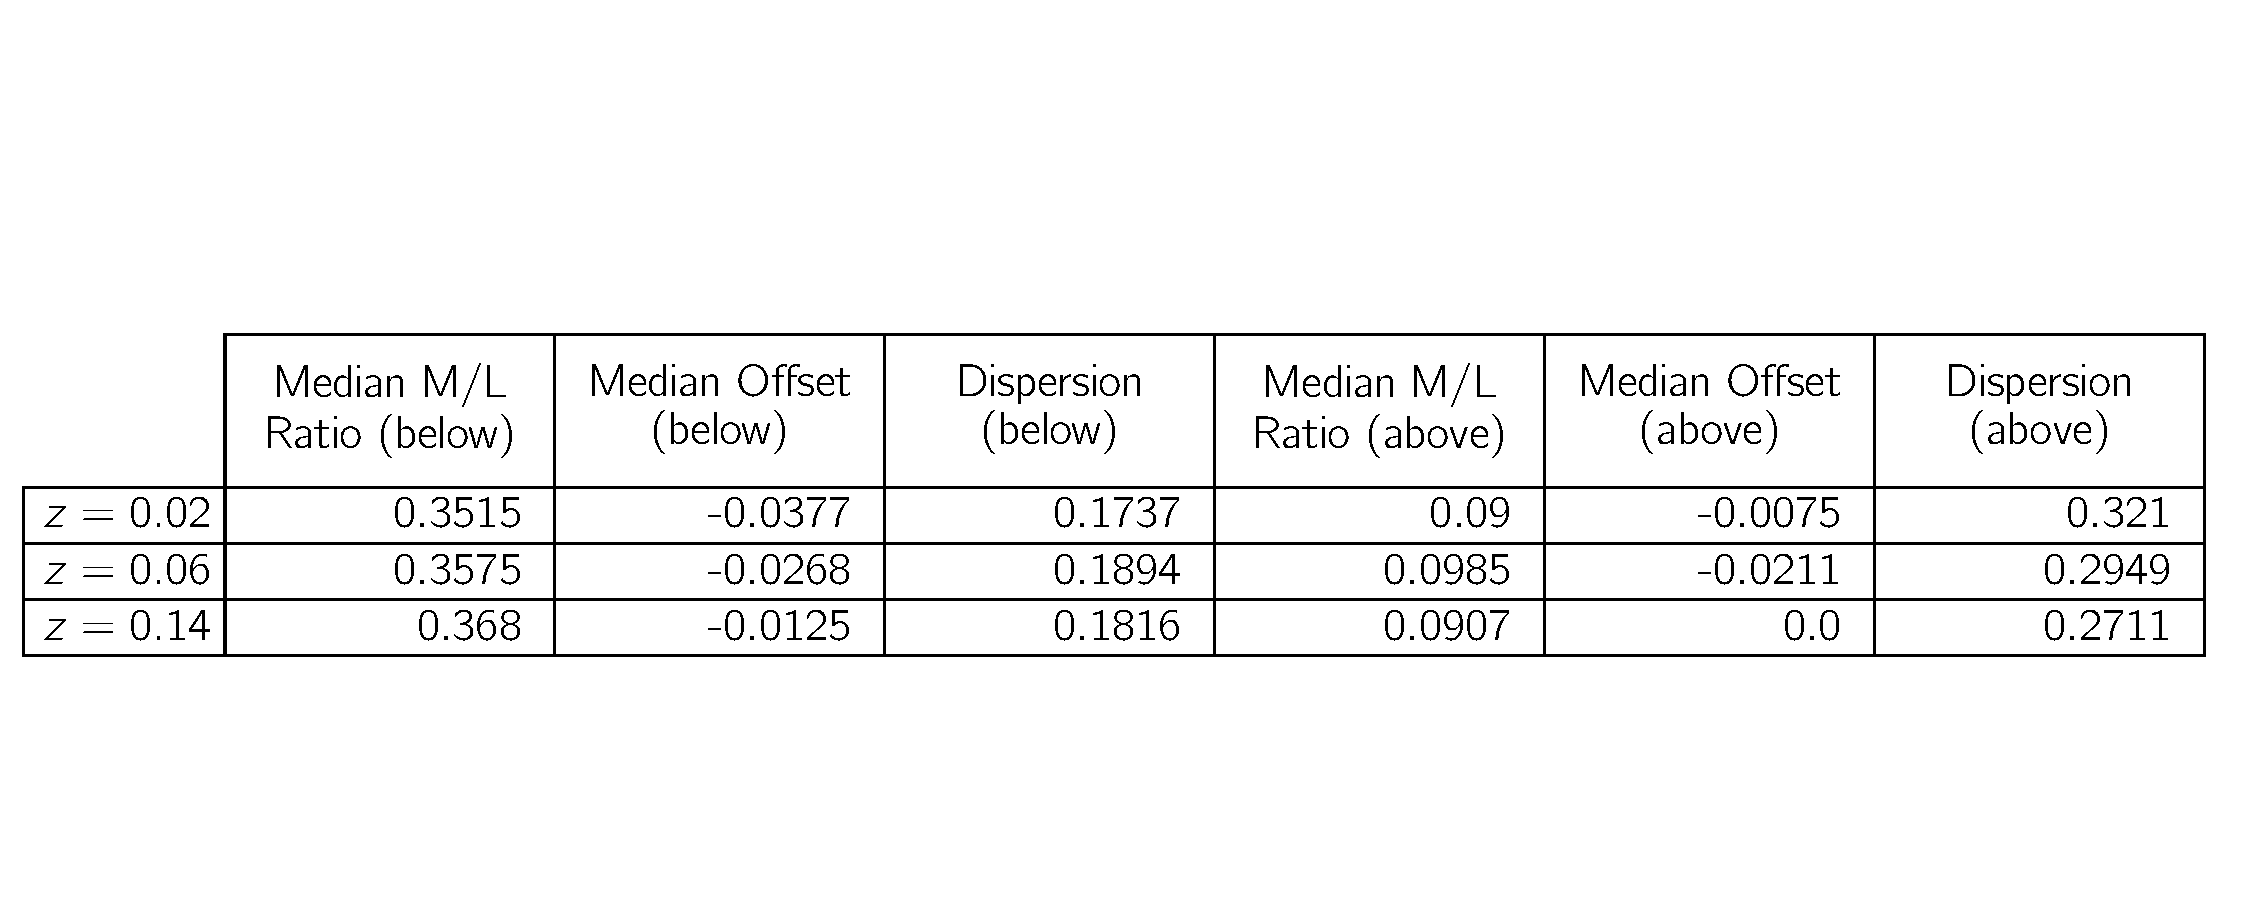
\includegraphics[width=\textwidth]{figures/table_median.pdf}
\caption[Table showing the median offsets for the three redshift bins.]
{Table showing the median offsets for the three redshift bins
\label{tab: median_offsets}}
\end{figure}

The fact that the mean offsets from the the full aperture measurements 
are small implies that the mean MPA-JHU masses are robust. These 
measurements are therefore not likely to cause an overall shift in the
measured stellar mass function, for example. 

However, the standard deviations are interestingly large. The scatter
this result implies in the stellar mass function is interesting for 
several reasons. First, it implies a correlation between the
stellar mass systematic error and the structure of galaxies, 
implying that galaxies with stronger bulges will have a slightly 
larger estimated mass. The standard deviation of 0.2 dex is still
small relative to the stellar mass bins defined by many analyses, 
but near the steep slope of the stellar mass function at high 
masses it may cause problems.

Second, this standard deviation, though small, is close to the 
standard deviation inferred between halo mass and stellar mass
for massive galaxies. For example, for BOSS galaxies
(which are further away and therefore less prone to 
aperture effects) \citealt{tinker17a} find around $\sim0.2$ dex 
standard deviation of stellar mass at fixed halo mass
based on their clustering. This result implies that a 
systematic error causing a 0.2 dex standard deviation 
(even with a mean of zero) is enough to affect similar analyses 
based on spectroscopic measurements with the SDSS Main Sample,
and therefore is a potential cause of concern for some 
applications.

Lastly, and related to both the previous points, this 0.2 dex 
standard deviation can affect the massive end of the stellar
mass function, causing the exponential cutoff at high masses 
to be less suddent than in reality.

In general, the results here suggest that some care may need 
to be taken in some contexts using the widely applied 
\citet{kauffmann_stellar_2003} 
results. Tables \ref{tab: mean_offset_table} 
and  \ref{tab: median_offsets} and Figure \ref{dispersion_plot} yield 
the quantitative description necessary to determine in which 
contexts these effects become important. Exactly how to account for
them will depend on the population of galaxies being studied, in 
particular their redshift, color, and mass selection. 

A similar set of concerns may affect the \citet{brinchmann_physical_2004} results
in the MPA-JHU catalog regarding star formation rates. 
These effects can be estimated using techniques similar to those
I use here.


%MRB Says: * This mean tendency is *relatively* small. You should calculate from your grids the median offset for cells with D4000 > 1.3 or something like that, and quote that number. You should then look carefully at the Kauffmann figure to translate this to a change in $M/L_z$ --- my guess is that it is around 0.1 dex for z=0.06. Do this for z=0.06 and z=0.14.

% * The scatter about this mean is substantial relative to the mean. Again, calculate the median standard deviation over the cells with D4000 > 1.3 to quantify this. My guess is that it is  comparable to the mean itself. This means for individual galaxies the error can be a lot bigger. Again quote for both those redshifts.

% * The main conclusion is that stellar masses more accurate than 0.1 dex (or whatever you see in the mean offset) are not possible, and that the scatter in the offset means the precision is degraded as well. This source of error is important
%to keep in mind but is probably not fatal for samples at z=0.1
%from MPA/JHU --- most results done rely on stellar masses
%at that precision. Using this sample at lower redshift may be
%much more iffy.







